\documentclass[aspectratio=169,11pt]{beamer}
\usepackage{novogaia-theme}
\title{Learning to decode molecular structure}
\author{Wuhao}
\date{19 Sep 2026}
\begin{document}

% 01 / 60 seconds
\begin{frame}
\begin{tikzpicture}[remember picture,overlay,shift={(current page.south west)}]
\header{RESEARCH / 19 SEP 2026}{}
\node[anchor=north west,inner sep=0,font=\brandmedium\fontsize{27}{30}\selectfont,text width=10.5cm] at (.75,7.3) {Learning to decode\\molecular structure};
\node[anchor=north west,inner sep=0,align=left,text width=9.2cm] at (.75,4.86) {From mass spectra to molecules,\\through learned representations.};
\node[anchor=base west,inner sep=0,font=\brandmedium\fontsize{12}{15}\selectfont] at (11.5,5.10) {Wuhao};
\node[anchor=base west,inner sep=0,small] at (11.5,4.60) {19 Sep 2026};
\draw[line] (.75,4.04)--(15.25,4.04);
\spectrum{1.2}{2.48}{.52}
\draw[arr] (3.55,2.78)--(4.60,2.78);
\peaktokens{5.02}{2.48}{ink}
\node[tag] at (6.04,2.15) {Learn the evidence};
\draw[arr] (7.55,2.78)--(8.65,2.78);
\molecule{9.80}{2.78}{.40}
\node[anchor=west,inner sep=0,align=left,font=\brandmedium\fontsize{13}{16}\selectfont] at (11.5,2.78) {Predict.\\Represent.\\Retrieve.};
\source{Novogaia research · Mathematical detail in the appendix}
\end{tikzpicture}
\end{frame}

% 02 / 75 seconds
\begin{frame}
\begin{tikzpicture}[remember picture,overlay,shift={(current page.south west)}]
\header{01 / THE INVERSE PROBLEM}{A spectrum is evidence, not a structure}
\molecule{2.05}{4.95}{.7}
\node[tag] at (2.05,3.58) {$G=(V,A)$};
\draw[arr] (3.24,5.54)--node[above,small]{fragmentation}(6.1,5.54);
\draw[arr,dashed] (6.1,4.56)--node[below,small]{inverse problem}(3.24,4.56);
\spectrum{6.7}{4.13}{.9}
\node[tag] at (8.32,2.98) {$S=\{(m_i,I_i)\}_{i=1}^{N}$};
\node[small,anchor=base,inner sep=0] at (13.25,6.42) {Same formula: $F=\mathrm{C_6H_6O}$};
\coordinate (candidatefork) at (11.1,4.75);
\draw[arr] (10.32,4.75)--(candidatefork);
\draw[ink,line width=.55pt] (11.1,3.2)--(11.1,5.72);
\foreach \y in {5.72,4.46,3.2}{\draw[thinarr] (11.1,\y)--(11.91,\y);}
% Phenol, SMILES Oc1ccccc1. Alternating inner bonds retain line-angle clarity.
\begin{scope}[shift={(12.83,5.72)}]
 \draw[ink,line width=.7pt] (-.42,0)--(-.21,.364)--(.21,.364)--(.42,0)--(.21,-.364)--(-.21,-.364)--cycle;
 \draw[ink,line width=.55pt] (-.327,.016)--(-.167,.294) (.167,.294)--(.327,.016) (.17,-.284)--(-.17,-.284);
 \draw[ink,line width=.7pt] (.42,0)--(.73,0);
 \node[anchor=west,inner sep=0,small] at (.79,0) {OH};
\end{scope}
\node[anchor=base west,inner sep=0,tag] at (14.7,5.66) {$G_1$};
% Cyclohexa-2,4-dien-1-one, SMILES O=C1C=CC=CC1.
\begin{scope}[shift={(12.83,4.46)}]
 \draw[ink,line width=.7pt] (-.42,0)--(-.21,.364)--(.21,.364)--(.42,0)--(.21,-.364)--(-.21,-.364)--cycle;
 \draw[ink,line width=.55pt] (-.327,.016)--(-.167,.294) (.17,-.284)--(-.17,-.284);
 \draw[ink,line width=.55pt] (.42,.038)--(.75,.038) (.42,-.038)--(.75,-.038);
 \node[anchor=west,inner sep=0,small] at (.81,0) {O};
\end{scope}
\node[anchor=base west,inner sep=0,tag] at (14.7,4.40) {$G_2$};
% Hexa-2,4,5-trienal, SMILES O=CC=CC=C=C; the cumulated bonds are collinear.
\begin{scope}[shift={(12.65,3.12)}]
 \node[anchor=south east,inner sep=0,small] at (-.265,.157) {O};
 \draw[ink,line width=.55pt] (-.234,.179)--(.019,.031) (-.272,.113)--(-.019,-.031);
 \draw[ink,line width=.7pt] (0,0)--(.34,.20)--(.68,0)--(1.02,.20)--(1.36,0)--(1.70,-.20);
 \draw[ink,line width=.55pt] (.381,.141)--(.682,-.035) (1.061,.141)--(1.741,-.259);
 \node[fill=paper,inner sep=.65pt,font=\figurefont\fontsize{7.4}{8}\selectfont] at (1.36,0) {C};
\end{scope}
\node[anchor=base west,inner sep=0,tag] at (14.7,3.14) {$G_3$};
\node[anchor=west,inner sep=0,font=\fontsize{15}{18}\selectfont] at (1.03,2.63) {$\displaystyle\widehat G=\arg\max\nolimits_G p(G\mid S,F)$};
\takeaway{Same ingredients. Different connections.}
\source{Illustrative spectrum, not a matched experiment. Candidate graphs all have formula C\textsubscript{6}H\textsubscript{6}O (verified from their SMILES with RDKit); examples show structural ambiguity, not candidate prevalence.}
\end{tikzpicture}
\end{frame}

% 03 / 60 seconds
\begin{frame}
\begin{tikzpicture}[remember picture,overlay,shift={(current page.south west)}]
\header{01 / THE STRATEGY}{Two routes from evidence to identity}
% Data are shown as measured spectra and molecular graphs; boxes denote operations.
\node[anchor=west,inner sep=0,tag] at (.75,6.55) {Generate};
\spectrum{1.25}{5.02}{.48}
\node[box,minimum width=2.4cm,text width=2.1cm,minimum height=.80cm,inner sep=4pt] (genencoder) at (5.2,5.60) {Encoder $h$};
\node[box,minimum width=2.5cm,text width=2.2cm,minimum height=.80cm,inner sep=4pt] (generator) at (8.4,5.60) {Generate};
\draw[arr] (3.45,5.60)--(genencoder.west);\draw[arr] (genencoder.east)--(generator.west);
\node[inner sep=1.5pt] (genC1) at (11.80,5.40) {C};
\node[inner sep=1.5pt] (genC2) at (12.85,5.75) {C};
\node[inner sep=1.5pt] (genO) at (13.90,5.40) {O};
\draw[ink,line width=1pt] (genC1)--(genC2)--(genO);
\draw[arr] (generator.east)--(10.90,5.60);
\node[font=\fontsize{11.5}{14}\selectfont,inner sep=0] at (12.80,4.58) {$G\sim p_\theta(G\mid h,F)$};

\node[anchor=west,inner sep=0,tag] at (.75,4.24) {Retrieve};
\spectrum{1.25}{2.77}{.48}
\node[box,minimum width=2.4cm,text width=2.1cm,minimum height=.80cm,inner sep=4pt] (retencoder) at (5.2,3.35) {Pretrained $f$};
\node[box,minimum width=2.5cm,text width=2.2cm,minimum height=.80cm,inner sep=4pt] (ranker) at (8.4,3.35) {Rank};
\draw[arr] (3.45,3.35)--(retencoder.west);\draw[arr] (retencoder.east)--(ranker.west);
\draw[arr] (ranker.east)--(10.75,3.35);
\node[small,inner sep=0] at (13.0,4.05) {$\mathcal C(F)$};
\foreach \x/\label/\name in {11.40/C/retA,12.02/C/retB,12.64/O/retC,13.45/C/retD,14.07/O/retE,14.69/C/retF}{
 \node[small,inner sep=1pt] (\name) at (\x,3.35) {\label};}
\draw[ink,line width=.8pt] (retA)--(retB)--(retC);\draw[ink,line width=.8pt] (retD)--(retE)--(retF);
\node[small,inner sep=0] at (12.02,2.95) {$G_1$};\node[small,inner sep=0] at (14.07,2.95) {$G_2$};
\draw[ink,line width=.9pt] (11.30,2.72)--(12.74,2.72);
\node[font=\fontsize{10.5}{13}\selectfont,inner sep=0] at (11.92,2.30) {$\widehat G=\arg\max\nolimits_{G\in\mathcal C(F)}s(f(S),G)$};
\takeaway{Propose a molecule — or rank a supplied candidate pool.}
\source{This talk: fingerprint-based generation → large-scale pretraining → relational models → retrieval. Spectra and heavy-atom graphs are illustrative, not experimental matched pairs.}
\end{tikzpicture}
\end{frame}

% 04 / 90 seconds
\begin{frame}
\begin{tikzpicture}[remember picture,overlay,shift={(current page.south west)}]
\header{02 / GENERATING MOLECULES}{DiffMS: fix the atoms, denoise the bonds}
% Spectrum -> encoder -> continuous representation -> graph denoiser.
\spectrum{1.25}{5.11}{.52}
\node[box,minimum width=2.6cm,text width=2.3cm,minimum height=.95cm,inner sep=4pt] (diffencoder) at (5.25,5.82) {MIST-derived\\encoder};
\node[inner sep=0,font=\fontsize{9.5}{11}\selectfont] (diffembedding) at (8.15,5.82) {$\begin{pmatrix}h_1\\[-1pt]h_2\\[-1pt]\vdots\end{pmatrix}$};
\node[small,inner sep=0] at (8.15,6.55) {$h(S)$};
\node[box,minimum width=3.5cm,text width=3.2cm,minimum height=.95cm,inner sep=4pt] (diffdecoder) at (12.15,5.82) {Conditional graph\\denoiser};
\draw[arr] (3.51,5.82)--(diffencoder.west);
\draw[arr] (diffencoder.east)--([xshift=-.20cm]diffembedding.west);
\draw[arr] ([xshift=.20cm]diffembedding.east)--(diffdecoder.west);
% Fingerprint supervision is an auxiliary pretraining branch, not the inference condition.
\foreach \i/\shade in {0/100,1/0,2/100,3/100,4/0,5/0,6/100,7/0}{\draw[draw=ink,line width=.4pt,fill=ink!\shade] (4.38+\i*.22,4.89) rectangle +(.18,.24);}
\draw[thinarr,dashed] (diffencoder.south)--(5.25,5.13);
\node[small,anchor=west,inner sep=0] at (6.30,4.99) {$\mathcal L_{\rm fp}$ pretraining};
% An illustrative fixed heavy-atom inventory, with no learned atom identities.
\foreach \x/\label/\name in {10.85/C/fixedA,11.55/C/fixedB,12.25/C/fixedC,12.95/O/fixedD}{\node[circle,draw=ink,line width=.7pt,minimum size=.4cm,inner sep=0,small] (\name) at (\x,4.72) {\label};}
\draw[arr] (12.15,4.95)--(diffdecoder.south);
\node[small,inner sep=0] at (14.08,4.72) {$F{:}\ \mathrm C_3\mathrm H_8\mathrm O$};
\node[small,inner sep=0] at (11.90,4.25) {$V=V(F)$};
% The matrix trajectory uses that fixed atom order.
\foreach \i/\x in {0/1.30,1/3.50,2/5.70}{
 \node[small] at (\x+.49,4.28) {$A_{\ifnum\i=0 T\else\ifnum\i=1 t\else0\fi\fi}$};
 \foreach \a in {0,...,3}{\foreach \b in {0,...,3}{\pgfmathtruncatemacro{\shade}{ifthenelse(\a==\b,0,ifthenelse(\i==2,ifthenelse(abs(\a-\b)==1,25,0),mod(\a+\b+\a*\b+\i,5)*25))}\fill[ink!\shade] (\x+\a*.25,2.76+\b*.25) rectangle +(.23,.23);}}
}
\draw[arr] (2.46,3.25)--(3.32,3.25);\draw[arr] (4.66,3.25)--(5.52,3.25);
\node[small,rotate=90] at (.91,3.25) {atom $i$};\node[tinytext] at (1.79,3.89) {atom $j$};
\foreach \x/\shade/\lab in {1.2/0/none,2.36/25/single,3.52/50/double,4.68/75/triple,5.84/100/aromatic}{\draw[fill=ink!\shade,draw=line,line width=.35pt] (\x,2.37) rectangle +(.42,.2);\node[tinytext,font=\figurefont\fontsize{6.5}{8}\selectfont] at (\x+.21,2.16) {\lab};}
\node[anchor=west,inner sep=0,font=\fontsize{12}{15}\selectfont] at (7.55,3.62) {$\displaystyle p_\theta(A_0\mid h,F)=$};
\node[anchor=west,inner sep=0,font=\fontsize{11.5}{14}\selectfont] at (7.55,2.72) {$\displaystyle\sum_{A_{1:T}}p(A_T)\prod_{t=1}^{T}p_\theta(A_{t-1}\mid A_t,h,F)$};
\takeaway{Fixed heavy atoms. Learned bonds.}
\source{\href{https://arxiv.org/html/2502.09571v2}{DiffMS (2025), §§3.1–3.3}. Schematic, unmatched objects; fingerprints supervise pretraining, inference uses $h(S)$. Heavy-atom counts/types are fixed; implicit hydrogen counts can vary.}
\end{tikzpicture}
\end{frame}

% 05 / 75 seconds
\begin{frame}
\begin{tikzpicture}[remember picture,overlay,shift={(current page.south west)}]
\header{02 / GENERATING MOLECULES}{Our alternative: write the molecule as SMILES}
\spectrum{1.25}{5.02}{.54}
\node[box,minimum width=2.4cm,text width=2.1cm,minimum height=.85cm,inner sep=4pt] (arencoder) at (5.18,5.80) {MIST encoder};
\draw[arr] (3.58,5.80)--(arencoder.west);
% Probability-valued fingerprint dimensions, shown as a vector rather than a process box.
\foreach \i/\shade in {0/94,1/7,2/87,3/91,4/12,5/5,6/84,7/4,8/95,9/13}{\draw[draw=ink,line width=.4pt,fill=ink!\shade] (7.13+\i*.27,5.575) rectangle +(.23,.45);}
\node[small,inner sep=0] at (8.46,6.47) {$\hat f\in[0,1]^d$};
\node[box,minimum width=2.8cm,text width=2.5cm,minimum height=.85cm,inner sep=4pt] (ardecoder) at (13.0,5.80) {AR transformer};
\draw[arr] (arencoder.east)--(7.13,5.80);\draw[arr] (9.79,5.80)--(ardecoder.west);
% The decoder emits the complete token sequence; a brace attaches the output arrow to it.
\node[inner sep=0,font=\figurefont\fontsize{9.2}{11.5}\selectfont] (arprefix) at (2.50,4.07) {\texttt{C6H6O [SEP]}};
\foreach \i/\t in {0/O,1/c1,2/c,3/c,4/c,5/c,6/c1,7/EOS}{\node[inner sep=0,font=\figurefont\fontsize{11}{13}\selectfont] (artoken\i) at (4.55+\i*1.30,4.07) {\texttt{\t}};}
\draw[thinarr,shorten <=.12cm,shorten >=.12cm] (arprefix.east)--(artoken0.west);
\foreach \i/\j in {0/1,1/2,2/3,3/4,4/5,5/6,6/7}{\draw[thinarr,shorten <=.12cm,shorten >=.12cm] (artoken\i.east)--(artoken\j.west);}
\draw[ink,line width=.6pt,decorate,decoration={brace,amplitude=.10cm}] (4.18,4.52)--(14.22,4.52);
\draw[arr] (ardecoder.south)--(13.0,4.94)--(9.20,4.94)--(9.20,4.64);
\node[anchor=west,inner sep=0,font=\fontsize{12}{15}\selectfont] at (1.03,3.25) {$\textstyle p_\psi(s\mid\hat f,F)=\prod_{t=1}^{L}p_\psi(s_t\mid s_{<t},\hat f,F)$};
\node[anchor=west,inner sep=0,font=\fontsize{12}{15}\selectfont] at (1.03,2.43) {$\textstyle\mathcal L_{\rm AR}=-\sum\nolimits_t\log p_\psi(s_t\mid s_{<t},\hat f,F)$};
\takeaway{One molecule, one token at a time.}
\source{\href{https://www.nature.com/articles/s42256-023-00708-3}{MIST (2023)}; \href{https://github.com/Novogaia/md4/blob/e804f677c0a2a44cc5388cc303d1c9c51183091f/md4/models/diffusion/md4.py}{Novogaia/md4, ar branch, e804f677}. Fingerprint cross-attention and formula-prefix conditioning; phenol tokens and spectrum are illustrative. Fingerprint shade: white 0 → black 1.}
\end{tikzpicture}
\end{frame}

% 06 / 65 seconds
\begin{frame}
\begin{tikzpicture}[remember picture,overlay,shift={(current page.south west)}]
\header{02 / GENERATING MOLECULES}{Two decoders. Two kinds of constraints.}
\node[font=\figurefont\bfseries\fontsize{13}{15}\selectfont] at (4.05,6.5) {Graph diffusion};
\node[font=\figurefont\bfseries\fontsize{13}{15}\selectfont] at (11.85,6.5) {Autoregressive SMILES};
\draw[line,line width=.45pt] (7.95,6.5)--(7.95,2.2);
\node[inner sep=0,font=\fontsize{10.5}{13}\selectfont] (noisymatrix) at (2.2,5.06) {$\begin{pmatrix}0&2&0\\2&0&1\\0&1&0\end{pmatrix}$};
\node[inner sep=0,font=\fontsize{10.5}{13}\selectfont] (cleanmatrix) at (5.9,5.06) {$\begin{pmatrix}0&1&0\\1&0&1\\0&1&0\end{pmatrix}$};
\node[small,anchor=south,inner sep=0] at ([yshift=.14cm]noisymatrix.north) {$A_T$};
\node[small,anchor=south,inner sep=0] at ([yshift=.14cm]cleanmatrix.north) {$A_0$};
\draw[arr,shorten <=.18cm,shorten >=.18cm] (noisymatrix.east)--node[above,small]{$T\;\text{steps}$}(cleanmatrix.west);
\node[small] at (4.05,4.18) {$i,j\in(\mathrm C,\mathrm C,\mathrm O)$};
\foreach \x/\token/\index in {9.42/C/1,11.04/C/2,12.66/O/3,14.28/EOS/4}{
 \node[box,minimum width=.9cm,minimum height=.8cm,inner sep=3pt] (comparison\index) at (\x,5.06) {\token};
 \node[small] at (\x,5.98) {$s_{\index}$};
}
\foreach \i/\j in {1/2,2/3,3/4}{\draw[arr] (comparison\i.east)--(comparison\j.west);}
\node[small] at (11.85,4.18) {Sequential sampling};
\node[font=\fontsize{14}{17}\selectfont] at (4.05,3.50) {$X=X(F)$};
\node[small] at (4.05,3.04) {Fixed heavy atoms};
\node[font=\fontsize{11.5}{14}\selectfont] at (11.85,3.50) {$p(s\mid\hat f,F)=\prod_t p(s_t\mid s_{<t},\hat f,F)$};
\node[small] at (11.85,3.04) {Explicit likelihood};
\node[small] at (4.05,2.35) {Repeated global refinement};
\node[small] at (11.85,2.35) {$\operatorname{formula}(s)\stackrel{?}{=}F$\quad Validate syntax + formula};
\takeaway{Choose where to enforce chemical structure.}
\source{\href{https://arxiv.org/html/2502.09571v2}{DiffMS}; \href{https://github.com/Novogaia/md4/tree/ar}{Novogaia/md4, ar}. Schematic ethanol example; matrix rows/columns: C,C,O; 0=no bond, 1=single, 2=double. No latency comparison.}
\end{tikzpicture}
\end{frame}

% 07 / 65 seconds
\begin{frame}
\begin{tikzpicture}[remember picture,overlay,shift={(current page.south west)}]
\header{03 / LEARNING FROM RAW SPECTRA}{Use the unlabeled reservoir}
\draw[ink,line width=.7pt] (.95,3.03) rectangle (4.03,6.22);
\node[font=\figurefont\bfseries\fontsize{12}{14}\selectfont] at (2.49,6.52) {MassIVE};
\node[font=\brandmedium\fontsize{38}{40}\selectfont] at (2.49,5.46) {1B+};
\node[small] at (2.49,4.65) {Public spectra};
\foreach \y/\label in {4.14/S_1,3.78/S_2,3.42/S_N}{
 \node[anchor=west,small] at (1.17,\y) {$\label$};
 \foreach \x/\h in {1.91/.16,2.16/.08,2.43/.23,2.7/.12,2.98/.18,3.23/.07,3.5/.13}{\draw[ink,line width=.6pt] (\x,\y-.11)--+(0,\h);}
}
\coordinate (filterinput) at (4.9,4.9);\coordinate (filteroutput) at (6.65,4.9);
\draw[ink,line width=.7pt,fill=soft] (4.9,5.9)--(6.05,5.28)--(6.65,5.28)--(6.65,4.52)--(6.05,4.52)--(4.9,3.9)--cycle;
\node[small] at (5.45,4.9) {QC};
\node[small] at (5.75,3.47) {Deduplicate};
\draw[arr] (4.03,4.9)--(filterinput);
% The selected corpus is a stack of spectral records, not a process box.
\coordinate (dreamscorpuswest) at (7.88,5.80);
\coordinate (dreamscorpuseast) at (10.03,5.80);
\foreach \y in {5.45,5.80,6.15}{
 \foreach \x/\h in {7.96/.08,8.22/.16,8.48/.10,8.74/.23,9.00/.08,9.26/.15,9.52/.07,9.78/.13}{\draw[ink,line width=.6pt] (\x,\y-.10)--+(0,\h);}
}
\node[small,inner sep=0] at (9.05,5.04) {23.5M selected};
\node[font=\figurefont\bfseries\fontsize{12}{14}\selectfont] at (9.05,6.58) {DreaMS};
\node[box,minimum width=2.5cm,text width=2.2cm,minimum height=1cm,inner sep=4pt] (ourcorpus) at (9.05,3.2) {Our encoder};
\draw[ink,line width=.8pt] (filteroutput)--(7.30,4.9);
\draw[arr] (7.30,4.9)|-(dreamscorpuswest);\draw[arr] (7.30,4.9)|-(ourcorpus.west);
\node[small,inner sep=0] (richmetadata) at (9.05,4.35) {Richer metadata $a$};
\draw[arr] (richmetadata.south)--(ourcorpus.north);
\draw[arr] (dreamscorpuseast)--(10.75,5.8);
\node[anchor=west,inner sep=0,font=\fontsize{11.5}{14}\selectfont] at (11.05,6.02) {$\widehat m_M,\quad\widehat{\operatorname{order}}(t_a,t_b)$};
\node[anchor=west,inner sep=0,small,align=left] at (11.05,5.37) {Masked peaks\\Retention order};
\draw[arr] (ourcorpus.east)--(10.75,3.2);
\node[anchor=west,inner sep=0,font=\fontsize{14}{17}\selectfont] at (11.05,3.42) {$\widehat z_M\approx T(S)_M$};
\node[anchor=west,inner sep=0,small] at (11.05,2.82) {Latent targets};
\takeaway{More spectra. Fewer required structure labels.}
\source{\href{https://massive.ucsd.edu/ProteoSAFe/dataset.jsp?task=c4f2a2160dbd47148d703d2f519a103a}{MassIVE: 1.2B public MS/MS}; \href{https://www.nature.com/articles/s41587-025-02663-3}{DreaMS}; \href{https://dreams-docs.readthedocs.io/en/latest/tutorials/msdata.html}{GeMS-A10: 23,517,534}. Corpus opportunity differs from our run size; data-flow schematic.}
\end{tikzpicture}
\end{frame}

% 08 / 70 seconds
\begin{frame}
\begin{tikzpicture}[remember picture,overlay,shift={(current page.south west)}]
\header{03 / LEARNING FROM RAW SPECTRA}{The same molecule can be measured differently}
\spectrum{1.15}{4.95}{.66}
\node[tag] at (2.34,4.00) {$(m_i,I_i)\mapsto h_i$};
\node[box,minimum width=3.7cm,text width=3.4cm,minimum height=1.1cm,inner sep=4pt] (contextencoder) at (7.4,5.7) {Spectrum encoder};
\draw[arr] (3.90,5.7)--(contextencoder.west);
\peaktokens{11.95}{5.4}{ink}
\draw[arr] (contextencoder.east)--(11.95,5.7);
\node[tag] at (12.97,4.76) {$h_1,\ldots,h_N,h_{\rm CLS}$};
% Acquisition metadata are coordinates, not an extra model operation.
\node[inner sep=0,font=\fontsize{11}{14}\selectfont] (metadata) at (7.4,2.75) {$\bigl(a_1,a_2,\ldots,a_{28}\bigr)$};
\node[small,inner sep=0] at (7.4,2.17) {$a\in\mathbb R^{28}$};
\draw[arr] (metadata.north)--node[right,small]{$\gamma_a,\beta_a$}(contextencoder.south);
\foreach \y/\label in {3.25/Precursor · charge,2.75/Energy · instrument,2.25/Time · polarity}{\node[anchor=west,inner sep=0,small] at (1.15,\y) {\label};}
\draw[thinarr] (4.05,2.75)--(metadata.west);
\node[anchor=west,inner sep=0,font=\fontsize{11.3}{14}\selectfont] at (10.20,3.05) {$\displaystyle h'=(1+\gamma_a)\odot\bar h+\beta_a$};
\node[anchor=west,inner sep=0,font=\fontsize{10}{13}\selectfont] at (10.20,2.30) {$\displaystyle\bar h=\operatorname{RMSNorm}(h)$};
\takeaway{Interpret the peaks in their acquisition context.}
\source{\href{https://github.com/wchen99998/spectra-learning/blob/86c1a6795c1b7c747f0c7f6a70ecd5b6b6a071d8/spectra_learning/models/spectrum_metadata.py}{28-D metadata schema}: values, presence flags and categorical encodings. AdaLN-Zero: encoder\_jax.py. Modulation is schematic; residual gates omitted.}
\end{tikzpicture}
\end{frame}

% 09 / 65 seconds
\begin{frame}
\begin{tikzpicture}[remember picture,overlay,shift={(current page.south west)}]
\header{03 / TWO-STAGE PRETRAINING}{First learn a teacher. Then learn from it.}
\node[anchor=base west,inner sep=0,small] at (1.05,6.47) {01 / MAE — visible peaks};
\node[anchor=base west,inner sep=0,small] at (8.6,6.47) {02 / JEPA};
\node[box,text width=1.85cm,inner xsep=4pt,minimum height=.8cm] (mae) at (5.67,5.325) {MAE $T$};

\begin{scope}[shift={(1.15,4.9)}]
\draw[muted,line width=.5pt] (0,0)--(2.5,0);
\draw[muted,line width=.5pt] (0,0)--(0,.85);
\draw[ink,line width=.8pt] (0.22,0)--(0.22,0.2125);
\draw[ink,line width=.8pt] (0.49,0)--(0.49,0.4590);
\draw[ink,line width=.8pt] (1.07,0)--(1.07,0.2635);
\draw[ink,line width=.8pt] (1.34,0)--(1.34,0.5015);
\draw[ink,line width=.8pt] (1.97,0)--(1.97,0.2465);
\draw[ink,line width=.8pt] (2.28,0)--(2.28,0.4080);
\foreach \x in {0,1.25,2.5}{\draw[muted,line width=.4pt] (\x,0)--+(0,-.04);}
\node[anchor=base east,inner sep=0,tinytext] at (2.5,-.28) {$m/z$ (Th; schematic)};
\node[rotate=90,inner sep=0,tinytext] at (-.22,.425) {$I/I_{\max}$};
\end{scope}
\coordinate (visibleout) at (3.77,5.325);
\draw[arr] (visibleout)--(mae.west);
\node[box,text width=2.05cm,inner xsep=4pt,minimum height=.8cm] (teacher) at (9.95,5.325) {Teacher $T(S)$};
\draw[arr] (mae.east)--node[above=4pt,small]{freeze}(teacher.west);
\node[anchor=base,inner sep=0,small] at (13.3,6.16) {$Y=T(S)_M$};
\draw[draw=ink!50,fill=ink!20,line width=.45pt] (12.400,5.030) rectangle +(.25,.24);
\draw[draw=ink!50,fill=ink!75,line width=.45pt] (12.710,5.030) rectangle +(.25,.24);
\draw[draw=ink!50,fill=ink!40,line width=.45pt] (13.020,5.030) rectangle +(.25,.24);
\draw[draw=ink!50,fill=ink!90,line width=.45pt] (13.330,5.030) rectangle +(.25,.24);
\draw[draw=ink!50,fill=ink!10,line width=.45pt] (13.640,5.030) rectangle +(.25,.24);
\draw[draw=ink!50,fill=ink!55,line width=.45pt] (13.950,5.030) rectangle +(.25,.24);
\draw[draw=ink!50,fill=ink!65,line width=.45pt] (12.400,5.380) rectangle +(.25,.24);
\draw[draw=ink!50,fill=ink!25,line width=.45pt] (12.710,5.380) rectangle +(.25,.24);
\draw[draw=ink!50,fill=ink!85,line width=.45pt] (13.020,5.380) rectangle +(.25,.24);
\draw[draw=ink!50,fill=ink!35,line width=.45pt] (13.330,5.380) rectangle +(.25,.24);
\draw[draw=ink!50,fill=ink!70,line width=.45pt] (13.640,5.380) rectangle +(.25,.24);
\draw[draw=ink!50,fill=ink!15,line width=.45pt] (13.950,5.380) rectangle +(.25,.24);
\coordinate (targetwest) at (12.3,5.325);
\coordinate (targetnorth) at (13.3,5.65);
\coordinate (targetsouth) at (13.3,5.0);
\draw[arr] (teacher.east)--(targetwest);
\node[anchor=base,inner sep=0,font=\fontsize{10}{12}\selectfont] at (9.95,4.43) {$\dot\theta_T=0$};
% A probability histogram is the MAE's output object.
\draw[muted,line width=.5pt] (1.55,2.69)--(3.80,2.69);
\draw[muted,line width=.5pt] (1.55,2.69)--(1.55,3.7);
\foreach \y/\lab in {2.69/0,3.59/0.3}{\draw[muted,line width=.4pt] (1.55,\y)--+(-.04,0);\node[tinytext,anchor=east,inner sep=1pt] at (1.46,\y) {\lab};}
\foreach \i/\h in {0/.06,1/.09,2/.24,3/.75,4/.9,5/.45,6/.15,7/.36}{\fill[ink] (1.70+\i*.24,2.69) rectangle +(.16,\h);}
\node[anchor=base,inner sep=0,small] at (2.7,3.98) {$p(b)$};
\node[anchor=base,inner sep=0,small] at (2.7,2.21) {Mass bins};
\draw[arr] (mae.south)--(5.67,3.16)--(4.03,3.16);
\node[anchor=base,inner sep=0,font=\fontsize{11}{13}\selectfont] at (5.55,2.22) {$\mathcal L_{\rm MAE}=\mathrm{CE}(p,b)$};
\node[box,text width=2.75cm,inner xsep=4pt,minimum height=.85cm] (student) at (9.95,3.15) {$g(f(C),Q)$};
\node[anchor=base,inner sep=0,small] at (9.95,3.96) {Student};
\draw[draw=ink!50,fill=ink!20,line width=.45pt] (12.400,2.855) rectangle +(.25,.24);
\draw[draw=ink!50,fill=ink!78,line width=.45pt] (12.710,2.855) rectangle +(.25,.24);
\draw[draw=ink!50,fill=ink!40,line width=.45pt] (13.020,2.855) rectangle +(.25,.24);
\draw[draw=ink!50,fill=ink!93,line width=.45pt] (13.330,2.855) rectangle +(.25,.24);
\draw[draw=ink!50,fill=ink!10,line width=.45pt] (13.640,2.855) rectangle +(.25,.24);
\draw[draw=ink!50,fill=ink!58,line width=.45pt] (13.950,2.855) rectangle +(.25,.24);
\draw[draw=ink!50,fill=ink!65,line width=.45pt] (12.400,3.205) rectangle +(.25,.24);
\draw[draw=ink!50,fill=ink!28,line width=.45pt] (12.710,3.205) rectangle +(.25,.24);
\draw[draw=ink!50,fill=ink!85,line width=.45pt] (13.020,3.205) rectangle +(.25,.24);
\draw[draw=ink!50,fill=ink!38,line width=.45pt] (13.330,3.205) rectangle +(.25,.24);
\draw[draw=ink!50,fill=ink!70,line width=.45pt] (13.640,3.205) rectangle +(.25,.24);
\draw[draw=ink!50,fill=ink!18,line width=.45pt] (13.950,3.205) rectangle +(.25,.24);
\coordinate (predictionwest) at (12.3,3.15);
\coordinate (predictionnorth) at (13.3,3.475);
\coordinate (predictionsouth) at (13.3,2.825);
\draw[arr] (student.east)--(predictionwest);
\draw[ink,line width=.7pt] (predictionnorth)--node[right=4pt,small]{MSE}(targetsouth);
\node[anchor=base,inner sep=0,font=\fontsize{10.5}{13}\selectfont] at (11.9,2.22) {$\mathcal L_{\rm JEPA}=\|\widehat Y-Y\|^2$};
\takeaway{Reconstruct measured peaks → predict learned meaning.}
\source{Implementation: configs/1b\_mae\_teacher\_jepa.py and 1p8b\_mae\_teacher\_jepa.py. Related two-stage idea: \href{https://arxiv.org/abs/2509.24317}{SALT}; our objective uses MSE. Objects are schematic.}
\end{tikzpicture}
\end{frame}

% 10 / 85 seconds
\begin{frame}
\begin{tikzpicture}[remember picture,overlay,shift={(current page.south west)}]
\header{03 / STAGE 1 — MAE}{Reconstruct mass, at more than one resolution}
\foreach \i/\v in {0/0,1/1,2/0,3/1,4/0,5/0}{
 \ifnum\v=1\node[box,ghost,minimum width=.5cm,minimum height=.75cm,inner sep=0] (maetoken\i) at (1.2+\i*.7,5.85) {?};
 \else\node[box,fill=ink,minimum width=.5cm,minimum height=.75cm,inner sep=0] (maetoken\i) at (1.2+\i*.7,5.85) {};\fi}
\node[box,minimum width=3.4cm,text width=3.1cm,minimum height=.85cm,inner sep=4pt] (maedecoder) at (8.1,5.85) {Encoder + decoder};
\draw[arr] (maetoken5.east)--(maedecoder.west);
\node[anchor=west,inner sep=0,align=left,small] (massbins) at (11.15,5.85) {$p_i(k)$\\masked mass bins};
\draw[arr] (maedecoder.east)--([xshift=-.15cm]massbins.west);
\node[tag] at (2.95,5.08) {Visible + masked};
\foreach \i/\shade in {0/2,1/3,2/4,3/6,4/10,5/15,6/20,7/15,8/10,9/6,10/5,11/4}{\fill[ink!\shade] (1.14+\i*.44,4.0) rectangle +(.41,.45);}
\foreach \i/\shade in {0/5,1/10,2/25,3/35,4/16,5/9}{\fill[ink!\shade] (1.14+\i*.88,3.25) rectangle +(.85,.4);}
\foreach \i/\shade in {0/15,1/60,2/25}{\fill[ink!\shade] (1.14+\i*1.76,2.62) rectangle +(1.73,.33);}
\foreach \y/\label in {4.225/fine,3.45/coarse,2.785/coarser}{\node[anchor=west,inner sep=0,small] at (6.70,\y) {\label};}
\node[anchor=west,inner sep=0,small] at (1.14,2.15) {Probability: white $0$ → black $1$};
\node[anchor=west,inner sep=0,font=\fontsize{12}{15}\selectfont] at (8.50,4.25) {$\displaystyle p_i^{(r)}(b)=\sum\nolimits_{k\in\mathcal B_r(b)}p_i(k)$};
\node[anchor=west,inner sep=0,font=\fontsize{12}{15}\selectfont] at (8.50,3.28) {$\displaystyle\mathcal L_{\rm MAE}=\sum\nolimits_r\lambda_r\,\mathrm{CE}(p_i^{(r)},b_i^{(r)})$};
\node[anchor=west,inner sep=0,font=\fontsize{10}{13}\selectfont] at (8.50,2.35) {$\displaystyle b_i^{(r)}=\lfloor b_i/r\rfloor,\quad r=1,2,4,\ldots$};
\takeaway{One distribution. Multiple resolutions.}
\source{Teacher recipe: 0.5 m/z-unit fine bins; multiscale marginal cross-entropy. Loss averaged over masked peaks; intensity reconstruction weight is zero in this recipe.}
\end{tikzpicture}
\end{frame}

% 11 / 90 seconds
\begin{frame}
\begin{tikzpicture}[remember picture,overlay,shift={(current page.south west)}]
\header{03 / STAGE 2 — FROZEN JEPA}{Predict what the teacher sees in the missing peaks}
\node[anchor=base,inner sep=0,small] at (2.40,6.54) {Full spectrum $S$};
\begin{scope}[shift={(1.15,5.38)}]
\draw[muted,line width=.5pt] (0,0)--(2.5,0);
\draw[muted,line width=.5pt] (0,0)--(0,.85);
\draw[ink,line width=.8pt] (0.22,0)--(0.22,0.2125);
\draw[ink,line width=.8pt] (0.49,0)--(0.49,0.4590);
\draw[ink,line width=.8pt] (0.76,0)--(0.76,0.7905);
\draw[ink,line width=.8pt] (1.07,0)--(1.07,0.2635);
\draw[ink,line width=.8pt] (1.34,0)--(1.34,0.5015);
\draw[ink,line width=.8pt] (1.68,0)--(1.68,0.6800);
\draw[ink,line width=.8pt] (1.97,0)--(1.97,0.2465);
\draw[ink,line width=.8pt] (2.28,0)--(2.28,0.4080);
\draw[draw=ink,fill=paper,line width=.55pt] (0.76,0.7905) circle (.065);
\draw[draw=ink,fill=paper,line width=.55pt] (1.68,0.6800) circle (.065);
\foreach \x in {0,1.25,2.5}{\draw[muted,line width=.4pt] (\x,0)--+(0,-.04);}
\node[anchor=base east,inner sep=0,tinytext] at (2.5,-.28) {$m/z$ (Th; schematic)};
\node[rotate=90,inner sep=0,tinytext] at (-.22,.425) {$I/I_{\max}$};
\end{scope}
\coordinate (fullout) at (3.77,5.805);
\node[box,text width=2.05cm,inner xsep=4pt,minimum height=.80cm] (teacher) at (5.38,5.805) {Frozen $T$};
\draw[arr] (fullout)--(teacher.west);
\node[anchor=base,inner sep=0,font=\fontsize{10}{12}\selectfont] at (5.38,6.47) {$\dot\theta_T=0$};
\node[anchor=base,inner sep=0,small] at (13.15,6.47) {Masked targets $Y$};
\draw[draw=ink!50,fill=ink!20,line width=.45pt] (12.250,5.510) rectangle +(.25,.24);
\draw[draw=ink!50,fill=ink!75,line width=.45pt] (12.560,5.510) rectangle +(.25,.24);
\draw[draw=ink!50,fill=ink!40,line width=.45pt] (12.870,5.510) rectangle +(.25,.24);
\draw[draw=ink!50,fill=ink!90,line width=.45pt] (13.180,5.510) rectangle +(.25,.24);
\draw[draw=ink!50,fill=ink!10,line width=.45pt] (13.490,5.510) rectangle +(.25,.24);
\draw[draw=ink!50,fill=ink!55,line width=.45pt] (13.800,5.510) rectangle +(.25,.24);
\draw[draw=ink!50,fill=ink!65,line width=.45pt] (12.250,5.860) rectangle +(.25,.24);
\draw[draw=ink!50,fill=ink!25,line width=.45pt] (12.560,5.860) rectangle +(.25,.24);
\draw[draw=ink!50,fill=ink!85,line width=.45pt] (12.870,5.860) rectangle +(.25,.24);
\draw[draw=ink!50,fill=ink!35,line width=.45pt] (13.180,5.860) rectangle +(.25,.24);
\draw[draw=ink!50,fill=ink!70,line width=.45pt] (13.490,5.860) rectangle +(.25,.24);
\draw[draw=ink!50,fill=ink!15,line width=.45pt] (13.800,5.860) rectangle +(.25,.24);
\coordinate (targetwest) at (12.15,5.805);
\coordinate (targetnorth) at (13.15,6.13);
\coordinate (targetsouth) at (13.15,5.4799999999999995);
\draw[arr] (teacher.east)--node[above=4pt,small]{$T(S)_M$}(targetwest);
\node[anchor=base,inner sep=0,small] at (2.40,4.77) {Visible context $C$};
\begin{scope}[shift={(1.15,3.62)}]
\draw[muted,line width=.5pt] (0,0)--(2.5,0);
\draw[muted,line width=.5pt] (0,0)--(0,.85);
\draw[ink,line width=.8pt] (0.22,0)--(0.22,0.2125);
\draw[ink,line width=.8pt] (0.49,0)--(0.49,0.4590);
\draw[ink,line width=.8pt] (1.07,0)--(1.07,0.2635);
\draw[ink,line width=.8pt] (1.34,0)--(1.34,0.5015);
\draw[ink,line width=.8pt] (1.97,0)--(1.97,0.2465);
\draw[ink,line width=.8pt] (2.28,0)--(2.28,0.4080);
\foreach \x in {0,1.25,2.5}{\draw[muted,line width=.4pt] (\x,0)--+(0,-.04);}
\node[anchor=base east,inner sep=0,tinytext] at (2.5,-.28) {$m/z$ (Th; schematic)};
\node[rotate=90,inner sep=0,tinytext] at (-.22,.425) {$I/I_{\max}$};
\end{scope}
\coordinate (contextout) at (3.77,4.045);
\node[box,text width=2.05cm,inner xsep=4pt,minimum height=.80cm] (student) at (5.38,4.045) {Student $f_\theta$};
\draw[arr] (contextout)--(student.west);
% Context features are vectors, not a second learned operation.
\foreach \i/\shade in {0/30,1/80,2/50,3/15}{\draw[draw=ink!50,fill=ink!\shade,line width=.45pt] (7.04+\i*.19,3.725) rectangle +(.13,.64);}
\node[anchor=base,inner sep=0,small] at (7.39,4.66) {$Z$};
\node[anchor=base,inner sep=0,font=\fontsize{10}{12}\selectfont] at (9.7,4.81) {$(\theta,\phi)\leftarrow\mathrm{optimize}$};
\draw[arr] (student.east)--(6.91,4.045);
\node[box,text width=2.45cm,inner xsep=4pt,minimum height=.80cm] (predictor) at (9.7,4.045) {$g_\phi(Z,Q)$};
\draw[arr] (7.91,4.045)--(predictor.west);
\draw[draw=ink!50,fill=ink!20,line width=.45pt] (12.250,3.750) rectangle +(.25,.24);
\draw[draw=ink!50,fill=ink!78,line width=.45pt] (12.560,3.750) rectangle +(.25,.24);
\draw[draw=ink!50,fill=ink!40,line width=.45pt] (12.870,3.750) rectangle +(.25,.24);
\draw[draw=ink!50,fill=ink!93,line width=.45pt] (13.180,3.750) rectangle +(.25,.24);
\draw[draw=ink!50,fill=ink!10,line width=.45pt] (13.490,3.750) rectangle +(.25,.24);
\draw[draw=ink!50,fill=ink!58,line width=.45pt] (13.800,3.750) rectangle +(.25,.24);
\draw[draw=ink!50,fill=ink!65,line width=.45pt] (12.250,4.100) rectangle +(.25,.24);
\draw[draw=ink!50,fill=ink!28,line width=.45pt] (12.560,4.100) rectangle +(.25,.24);
\draw[draw=ink!50,fill=ink!85,line width=.45pt] (12.870,4.100) rectangle +(.25,.24);
\draw[draw=ink!50,fill=ink!38,line width=.45pt] (13.180,4.100) rectangle +(.25,.24);
\draw[draw=ink!50,fill=ink!70,line width=.45pt] (13.490,4.100) rectangle +(.25,.24);
\draw[draw=ink!50,fill=ink!18,line width=.45pt] (13.800,4.100) rectangle +(.25,.24);
\coordinate (predictionwest) at (12.15,4.045);
\coordinate (predictionnorth) at (13.15,4.37);
\coordinate (predictionsouth) at (13.15,3.72);
\draw[arr] (predictor.east)--(predictionwest);
\node[anchor=base,inner sep=0,small] at (13.15,3.31) {$\widehat Y$};
\draw[ink,line width=.7pt] (predictionnorth)--node[right=4pt,small]{MSE}(targetsouth);
\node[anchor=base west,inner sep=0,font=\fontsize{12}{15}\selectfont] at (1.05,2.53) {$\displaystyle Y=\sg[\mathcal N(T(S)_M)],\qquad\mathcal L_{\rm JEPA}=\frac{1}{|M|d}\sum_{i\in M}\|\widehat Y_i-Y_i\|_2^2$};
\takeaway{Deploy the student encoder $f_\theta$.}
\source{$M$: target peaks; $Q$: target-query information; $\mathcal N$: target normalization (identity here). Frozen teacher, no EMA. Acquisition metadata conditions the model. Circles: masked targets. Traces/colors are schematic; shared pre-mask intensity scale.}
\end{tikzpicture}
\end{frame}

% 12 / 80 seconds
\begin{frame}
\begin{tikzpicture}[remember picture,overlay,shift={(current page.south west)}]
\header{04 / WHY THE STUDENT CAN DIFFER}{Same teacher target. Different student codes.}
% A fixed teacher defines the same scalar target for this one input.
\node[small,anchor=base,inner sep=0] at (2.5,6.64) {Same spectrum $S$};
\draw[muted,line width=.55pt] (1.42,5.80)--(3.55,5.80);
\draw[muted,line width=.55pt] (1.42,5.80)--(1.42,6.48);
\foreach \x/\h in {.16/.16,.36/.48,.58/.25,.82/.60,1.06/.19,1.27/.40,1.52/.22,1.81/.30,1.98/.16}{\draw[ink,line width=.8pt] (1.42+\x,5.80)--+(0,\h);}
\node[tinytext,anchor=north,inner sep=1pt] at (2.49,5.73) {$m/z$ (Th; schematic)};
\node[tinytext,rotate=90,inner sep=0] at (1.14,6.14) {$I/I_{\max}$};
\node[box,minimum width=2.45cm,minimum height=.66cm,inner sep=4pt] (teacher) at (7.68,6.15) {Frozen teacher $T$};
\draw[arr] (3.85,6.15)--(teacher.west);
\node[small,anchor=base,inner sep=0] at (12.18,6.67) {Fixed target $Y$};
\draw[ink,fill=soft,line width=.65pt] (11.73,5.80) rectangle (12.63,6.50);
\node[font=\fontsize{16}{19}\selectfont,inner sep=0] at (12.18,6.15) {$4$};
\draw[arr] (teacher.east)--(11.58,6.15);
% Two equally valid student/predictor factorizations, not a training sequence.
\node[small,anchor=base,inner sep=0] at (2.77,5.01) {Student code $Z$};
\node[small,anchor=base,inner sep=0] at (7.68,5.01) {Predictor $g$};
\node[small,anchor=base,inner sep=0] at (12.18,5.01) {Prediction $\widehat Y$};
\foreach \y/\name/\code/\operation in {4.34/A/2/{\times 2},3.11/B/8/{\div 2}}{
 \node[small,anchor=west,inner sep=0] at (1.05,\y) {Code \name};
 \draw[ink,fill=soft,line width=.65pt] (2.63,\y-.35) rectangle (3.53,\y+.35);
 \node[font=\fontsize{16}{19}\selectfont,inner sep=0] at (3.08,\y) {$\code$};
 \node[box,minimum width=2.45cm,minimum height=.70cm,inner sep=4pt] (pred\name) at (7.68,\y) {$\operation$};
 \draw[arr] (3.68,\y)--(pred\name.west);
 \draw[ink,fill=soft,line width=.65pt] (11.73,\y-.35) rectangle (12.63,\y+.35);
 \node[font=\fontsize{16}{19}\selectfont,inner sep=0] at (12.18,\y) {$4$};
 \draw[arr] (pred\name.east)--(11.58,\y);}
\draw[muted,dashed,line width=.65pt] (12.80,6.15)--(13.45,6.15)--(13.45,3.11)--(12.80,3.11);
\draw[muted,dashed,line width=.65pt] (12.80,4.34)--(13.45,4.34);
\node[small,anchor=west,inner sep=0,align=left] at (13.73,4.69) {Both\\match};
\node[anchor=base,inner sep=0,font=\fontsize{12}{15}\selectfont] at (8.02,2.23) {$\widehat Y=g(Z),\qquad\mathcal L=\tfrac12(\widehat Y-Y)^2$};
\takeaway{Freezing fixes each input’s target; the student can use a different code.}
\source{One-feature toy example: arbitrary values, not measured features. Two possible factorizations of the same prediction, not successive training steps. Freezing alone does not guarantee a better or different representation. General argument: Appendix I.}
\end{tikzpicture}
\end{frame}

% 13 / 75 seconds
\begin{frame}
\begin{tikzpicture}[remember picture,overlay,shift={(current page.south west)}]
\header{04 / WHY THE TRAINING WORKS}{When the answer is uncertain, predict its average}
% One visible context; no mark, placeholder or mass hint for the withheld peak.
\node[small,inner sep=0] at (2.30,5.74) {Visible context $C$};
\node[tinytext,anchor=west,inner sep=0] at (1.25,5.22) {Relative intensity (a.u.)};
\begin{scope}[shift={(1.25,4.25)}]
 \draw[muted,line width=.5pt] (0,0)--(2.10,0);\draw[muted,line width=.5pt] (0,0)--(0,.72);
 \foreach \x/\h in {.22/.25,.55/.56,.86/.34,1.61/.41,1.88/.22}{\draw[ink,line width=.85pt] (\x,0)--+(0,\h);}
 \foreach \x/\lab in {0/0,1.05/150,2.1/300}{\draw[muted,line width=.45pt] (\x,0)--+(0,-.04);\node[anchor=north,inner sep=1pt,font=\figurefont\fontsize{6}{7}\selectfont] at (\x,-.07) {\lab};}
 \foreach \y/\lab in {0/0,.70/1}{\node[anchor=east,inner sep=1pt,font=\figurefont\fontsize{6}{7}\selectfont] at (-.05,\y) {\lab};}
 \node[anchor=north east,inner sep=0,tinytext] at (2.10,-.39) {$m/z$ (Th)};
\end{scope}
\node[small,inner sep=0,align=center] at (2.30,3.18) {Same visible peaks\\Same query $Q$};
% Dashed forks denote alternative full inputs, not teacher drift through time.
\draw[thinarr,dashed] (3.70,4.61)--(4.12,4.61);
\draw[muted,dashed,line width=.55pt] (4.12,3.28)--(4.12,5.94);
\node[small,inner sep=0] at (6.15,6.61) {Possible full spectra};
\node[small,inner sep=0] at (8.45,6.61) {Fixed $T$};
\node[small,inner sep=0] at (10.15,6.61) {Feature (a.u.)};
\foreach \base/\hiddenx/\hiddenh/\value/\idx in {5.58/1.05/.65/8/1,4.25/1.22/.31/10/2,2.92/1.41/.48/12/3}{
 \pgfmathsetmacro{\cy}{\base+.36}
 \draw[thinarr,dashed] (4.12,\cy)--node[above,inner sep=1pt,tinytext] {$1/3$}(4.88,\cy);
 \begin{scope}[shift={(5.10,\base)}]
  \draw[muted,line width=.5pt] (0,0)--(2.10,0);\draw[muted,line width=.5pt] (0,0)--(0,.72);
  \foreach \x/\h in {.22/.25,.55/.56,.86/.34,1.61/.41,1.88/.22}{\draw[ink,line width=.85pt] (\x,0)--+(0,\h);}
  \draw[muted,dashed,line width=1pt] (\hiddenx,0)--+(0,\hiddenh);
  \foreach \x/\lab in {0/0,1.05/150,2.1/300}{\draw[muted,line width=.45pt] (\x,0)--+(0,-.04);\node[anchor=north,inner sep=1pt,font=\figurefont\fontsize{6}{7}\selectfont] at (\x,-.07) {\lab};}
  \foreach \y/\lab in {0/0,.70/1}{\node[anchor=east,inner sep=1pt,font=\figurefont\fontsize{6}{7}\selectfont] at (-.05,\y) {\lab};}
 \end{scope}
 \node[box,minimum width=1.12cm,minimum height=.62cm,inner sep=3pt] (teacher\idx) at (8.45,\cy) {$T$};
 \draw[arr] (7.42,\cy)--(teacher\idx.west);
 \node[draw=ink,fill=paper,line width=.7pt,minimum width=.72cm,minimum height=.62cm,inner sep=0,font=\figurefont\fontsize{14}{16}\selectfont] (feature\idx) at (10.15,\cy) {\value};
 \draw[arr] (teacher\idx.east)--(feature\idx.west);
 \draw[ink,line width=.65pt] (feature\idx.east)--(11.22,\cy);
}
\node[anchor=north east,inner sep=0,tinytext] at (7.20,2.54) {$m/z$ (Th)};
\draw[muted,dashed,line width=1pt] (1.25,2.35)--(1.67,2.35);
\node[anchor=west,inner sep=0,tinytext] at (1.82,2.35) {Withheld peak};
% A conditional mean: the three teacher outputs are equally probable given C,Q.
\draw[ink,line width=.65pt] (11.22,3.28)--(11.22,5.94);
\node[draw=ink,fill=soft,line width=.7pt,minimum width=1.20cm,minimum height=1.04cm,inner sep=0,font=\figurefont\fontsize{28}{30}\selectfont] (bestprediction) at (13.22,4.61) {10};
\draw[arr] (11.22,4.61)--(bestprediction.west);
\node[small,inner sep=0,align=center] at (13.22,5.87) {Best squared-error\\prediction};
\node[inner sep=0,font=\fontsize{11}{14}\selectfont] at (13.22,3.47) {$(8+10+12)/3=10$};
\node[anchor=west,inner sep=0,font=\fontsize{10.5}{13}\selectfont] at (9.65,2.28) {$\widehat Y^*=\mathbb E[Y\mid C,Q]=10$};
\takeaway{Learn what the visible evidence can support.}
\source{Attached analysis: conditional expectation under squared error. Synthetic equally likely completions, fixed $C,Q,T$; values are one learned feature, not mass or intensity. Predictable need not mean chemical; no student-over-teacher guarantee.}
\end{tikzpicture}
\end{frame}

% 14 / 90 seconds
\begin{frame}
\begin{tikzpicture}[remember picture,overlay,shift={(current page.south west)}]
\header{04 / TRAINING DYNAMICS}{The predictor directs the student’s learning}
% Explicit code coordinates: the predictor reads z_1 and ignores z_2.
\node[small,anchor=base,inner sep=0] at (2.20,6.43) {Code $Z$};
\draw[draw=ink,fill=soft,line width=.65pt] (1.60,5.25) rectangle (2.80,6.00);
\draw[draw=ink,fill=paper,line width=.65pt] (1.60,4.50) rectangle (2.80,5.25);
\node[anchor=east,inner sep=0,small] at (1.38,5.625) {$z_1$};
\node[anchor=east,inner sep=0,small] at (1.38,4.875) {$z_2$};
\node[font=\fontsize{20}{22}\selectfont,inner sep=0] at (2.20,5.625) {$1$};
\node[font=\fontsize{20}{22}\selectfont,inner sep=0] at (2.20,4.875) {$5$};
\node[anchor=base west,inner sep=0,small] at (.95,3.93) {No direct feedback to $z_2$};
% Only the model operation is boxed. Forward and backward ports are separate.
\node[box,text width=2.55cm,inner xsep=4pt,minimum height=.95cm] (predictor) at (5.70,5.625) {$g(Z)=2z_1$};
\node[small,anchor=base,inner sep=0] at (5.70,6.43) {Predictor};
\draw[arr] (2.80,5.83)--(predictor.west |- 0,5.83);
\draw[arr] (predictor.west |- 0,5.40)--(2.80,5.40);
\node[anchor=base,inner sep=0,font=\fontsize{11}{13}\selectfont] at (3.54,5.04) {$-4$};
% Numerical comparison of the prediction with the fixed teacher target.
\node[font=\fontsize{24}{27}\selectfont,inner sep=3pt] (prediction) at (9.15,5.625) {$2$};
\node[font=\fontsize{24}{27}\selectfont,inner sep=3pt] at (10.28,5.625) {$-$};
\node[font=\fontsize{24}{27}\selectfont,inner sep=3pt] at (11.40,5.625) {$4$};
\node[font=\fontsize{20}{24}\selectfont,inner sep=3pt] at (12.60,5.625) {$=$};
\node[font=\fontsize{24}{27}\selectfont,inner sep=3pt] (error) at (14.00,5.625) {$-2$};
\node[small,anchor=base,inner sep=0] at (9.15,6.43) {Prediction};
\node[small,anchor=base,inner sep=0] at (11.40,6.43) {Fixed teacher};
\node[small,anchor=base,inner sep=0] at (14.00,6.43) {Error};
\draw[arr] (predictor.east)--(prediction.west);
\draw[arr] (error.south)--(14.00,4.20)--node[above=4pt,small]{error feedback}(5.70,4.20)--(predictor.south);
\node[anchor=base west,inner sep=0,font=\fontsize{13}{16}\selectfont] at (1.05,2.64) {$\displaystyle\frac{\partial\mathcal L}{\partial z_1}=2(2-4)=-4,\qquad\frac{\partial\mathcal L}{\partial z_2}=0$};
\node[anchor=west,inner sep=0,align=left,small] at (10.0,2.90) {To reduce the error:\\increase $z_1$.};
\takeaway{The learning signal passes through the predictor.}
\source{Toy illustration: fixed predictor $g(Z)=2z_1$, independent code coordinates, and $\mathcal L=\frac12(\widehat y-y)^2$. Shared encoder parameters can still move other code directions; zero direct gradient does not mean a coordinate never changes.}
\end{tikzpicture}
\end{frame}

% 15 / 90 seconds
\begin{frame}
\begin{tikzpicture}[remember picture,overlay,shift={(current page.south west)}]
\header{04 / TRAINING DYNAMICS}{Some predictable patterns are learned earlier}
\node[anchor=north west,inner sep=0] at (.8,6.48) {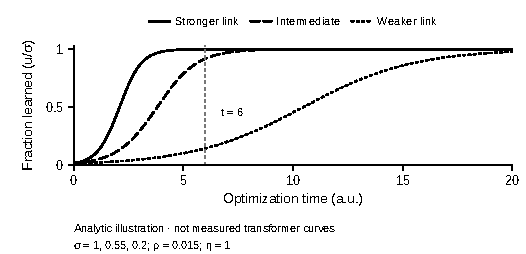
\includegraphics[width=8.75cm]{assets/dynamics-modes.pdf}};
\node[anchor=base west,inner sep=0,font=\figurefont\fontsize{10}{12}\selectfont] at (10.2,6.34) {Encoder + predictor};
\node[anchor=base west,inner sep=0,small] at (10.2,5.98) {Progress at the same time: $t=6$};
\node[anchor=base west,inner sep=0,small] at (10.2,5.52) {Stronger link};
\node[anchor=base east,inner sep=0,small] at (14.85,5.52) {$\approx 100\%$};
\path[fill=soft] (10.2,4.98) rectangle +(4.65,.26);
\path[fill=ink] (10.2,4.98) rectangle +(4.64812462,.26);
\draw[ink,line width=.55pt] (10.2,4.98) rectangle +(4.65,.26);
\node[anchor=base west,inner sep=0,small] at (10.2,4.60) {Intermediate};
\node[anchor=base east,inner sep=0,small] at (14.85,4.60) {$\approx 92\%$};
\path[fill=soft] (10.2,4.06) rectangle +(4.65,.26);
\path[fill=ink] (10.2,4.06) rectangle +(4.26867564,.26);
\draw[ink,line width=.55pt] (10.2,4.06) rectangle +(4.65,.26);
\node[anchor=base west,inner sep=0,small] at (10.2,3.68) {Weaker link};
\node[anchor=base east,inner sep=0,small] at (14.85,3.68) {$\approx 14\%$};
\path[fill=soft] (10.2,3.14) rectangle +(4.65,.26);
\path[fill=ink] (10.2,3.14) rectangle +(0.66837756,.26);
\draw[ink,line width=.55pt] (10.2,3.14) rectangle +(4.65,.26);
\node[anchor=base west,inner sep=0,small] at (10.2,2.63) {Time to reach 50\%};
\node[anchor=base east,inner sep=0,font=\fontsize{12}{15}\selectfont] at (14.85,2.63) {$t_{50\%}\propto 1/\sigma$};
\takeaway{Stronger context–target links can emerge earlier, even with fixed targets.}
\source{Ideal linear model: $u_i=a_i b_i$, progress $u_i/\sigma_i$. Centered, whitened context; aligned modes; balanced factors; equal rates; $u_i(0)=0.015\sigma_i$. $\sigma$: cross-covariance strength, including target scale. Analytic, not measured encoder utility. Attached analysis; \href{https://arxiv.org/abs/1312.6120}{Saxe et al.}.}
\end{tikzpicture}
\end{frame}

% 16 / 75 seconds
\begin{frame}
\begin{tikzpicture}[remember picture,overlay,shift={(current page.south west)}]
\header{04 / WHAT TO MEASURE}{Same loss does not mean the same representation}
\node[anchor=base west,inner sep=0,tag] at (1.0,6.42) {Proposed tests};
% Context is an illustrative sparse spectrum; no hidden peaks or numeric claims.
\node[anchor=base,inner sep=0,small] at (1.77,5.53) {Context $C$};
\draw[muted,line width=.5pt] (1.05,4.40)--(2.49,4.40);
\draw[muted,line width=.5pt] (1.05,4.40)--(1.05,5.20);
\foreach \x/\h in {1.20/.20,1.40/.65,1.67/.28,1.92/.47,2.16/.24,2.34/.55}{\draw[ink,line width=.75pt] (\x,4.40)--+(0,\h);}
\node[anchor=base,inner sep=0,font=\figurefont\fontsize{6.5}{8}\selectfont] at (1.80,4.05) {$m/z$ (Th; schematic)};
\node[rotate=90,inner sep=0,font=\figurefont\fontsize{6.5}{8}\selectfont] at (.88,4.80) {$I/I_{\max}$};
\node[box,text width=1.30cm,inner xsep=4pt,minimum height=.82cm] (encoder) at (3.70,4.8) {$f_\theta$};
\node[anchor=base,inner sep=0,small] at (3.70,5.53) {Frozen encoder};
\draw[arr] (2.62,4.80)--(encoder.west);
% A row of coordinate tiles represents the encoder output.
\foreach \x in {4.98,5.20,5.42}{\draw[draw=ink,fill=soft,line width=.55pt] (\x,4.48) rectangle +(.14,.64);}
\node[anchor=base,inner sep=0,small] at (5.27,5.53) {$Z$};
\draw[arr] (encoder.east)--(4.84,4.80);
\coordinate (latentright) at (5.56,4.80);
\coordinate (latentbottom) at (5.27,4.48);
\node[box,text width=1.45cm,inner xsep=4pt,minimum height=.82cm] (predictor) at (7.25,5.83) {$g_\phi$};
\node[small] at (7.25,6.48) {Predictor};
\node[box,text width=1.45cm,inner xsep=4pt,minimum height=.82cm] (readout) at (7.25,3.83) {$R_\psi$};
\node[small] at (7.25,3.15) {Fresh readout};
\draw[ink,line width=.55pt] (latentright)--(6.05,4.80);
\fill[ink] (6.05,4.80) circle (.04);
\draw[arr] (6.05,4.80)|-(predictor.west);
\draw[arr] (6.05,4.80)|-(readout.west);
\node[font=\fontsize{12}{14}\selectfont,inner sep=2pt] (loss) at (9.10,5.83) {$\mathcal L_{\rm JEPA}$};
\node[font=\fontsize{12}{14}\selectfont,inner sep=2pt] (hit) at (9.10,3.83) {$\mathrm{Hit@1}$};
\draw[arr] (predictor.east)--(loss.west);
\draw[arr] (readout.east)--(hit.west);
\node[anchor=base,inner sep=0] (variation) at (5.27,2.43) {$\operatorname{Cov}_{S}[Z],\quad r_{\rm eff}(Z)$};
\node[anchor=base east,inner sep=0,small] at (2.80,2.43) {Variation};
\draw[arr] (latentbottom)--([yshift=4pt]variation.north);
\draw[line,line width=.45pt] (10.0,6.47)--(10.0,2.19);
\node[small] at (12.86,6.47) {Independent controls};
\foreach \x in {11.45,12.35,13.25,14.15}{\draw[line,line width=.45pt] (\x,3.23)--(\x,5.93);}
\foreach \y in {3.23,4.13,5.03,5.93}{\draw[line,line width=.45pt] (11.45,\y)--(14.15,\y);}
\foreach \x in {11.90,12.80,13.70}{\foreach \y in {3.68,4.58,5.48}{\draw[ink,line width=.6pt,fill=paper] (\x,\y) circle (.09);}}
\draw[arr] (11.35,3.02)--(14.28,3.02);
\draw[arr] (11.23,3.14)--(11.23,6.03);
\node[anchor=base,inner sep=0,small] at (12.81,2.65) {Depth $L_p$};
\node[small,rotate=90] at (10.73,4.61) {Rate $\eta_p/\eta_e$};
\node[anchor=base,inner sep=0,small] at (12.82,2.16) {Fixed masks $\cdot$ matched compute};
\takeaway{Lower loss $\not\Rightarrow$ better retrieval.}
\source{Proposed diagnostics from the supplied analysis; no measured outcomes shown. Readout comparisons freeze encoder checkpoints. The depth/rate grid represents separate pretraining ablations, not simultaneous readout training. Spectrum and feature tiles are schematic.}
\end{tikzpicture}
\end{frame}

% 17 / 75 seconds
\begin{frame}
\begin{tikzpicture}[remember picture,overlay,shift={(current page.south west)}]
\header{05 / RELATIONAL REPRESENTATIONS}{Give each peak pair its own memory}
\node[anchor=base west,inner sep=0,small] at (1.05,6.4) {Single states $h_i$};
\foreach \i/\mass in {0/100,1/118,2/144,3/162}{
 \node[small] at (1.4,5.55-\i*.74) {\mass};
 \draw[fill=ink!20,draw=ink] (2.12,5.35-\i*.74) rectangle +(2.25,.4);}
\node[anchor=base,inner sep=0,small] at (1.4,2.77) {$m/z$ (Th)};
\draw[decorate,decoration={brace,amplitude=4pt},line width=.55pt] (4.61,5.55)--node[right=5pt,small]{$18$ Th}(4.61,4.81);
\draw[decorate,decoration={brace,amplitude=4pt},line width=.55pt] (4.61,4.07)--node[right=5pt,small]{$18$ Th}(4.61,3.33);
\draw[arr] (5.88,4.45)--(7.13,4.45);
\node[anchor=base,inner sep=0,small] at (8.7,6.4) {Pair states $Z_{ij}$};
\foreach \i in {0,...,3}{\foreach \j in {0,...,3}{\draw[draw=line,fill=soft,line width=.35pt] (7.4+\j*.64,3.2+\i*.64) rectangle +(.55,.55);}}
\node[anchor=base,inner sep=0,small] at (8.635,5.95) {$j$};
\node[anchor=east,inner sep=0,small] at (7.16,5.4) {$i$};
\draw[ink,line width=.7pt] (8.04,5.12) rectangle +(.55,.55);
\draw[arr] (10.13,4.45)--(10.9,4.45);
\node[anchor=west,inner sep=0,font=\fontsize{10}{13}\selectfont] at (11.1,4.45) {$\begin{aligned}Z_{ij}=\phi(&m_i-m_j,\\ &I_i,I_j,\ldots)\end{aligned}$};
\node[anchor=base west,inner sep=0,font=\fontsize{12}{15}\selectfont] at (1.05,2.26) {$N\times d_s\quad\longrightarrow\quad N\times N\times d_p$};
\takeaway{Equal mass gaps can have different contexts.}
\source{spectra\_learning/models/pairmixer\_jax.py. Single states already carry context; the pair stream stores relations explicitly. Peak masses here are illustrative.}
\end{tikzpicture}
\end{frame}

% 18 / 90 seconds
\begin{frame}
\begin{tikzpicture}[remember picture,overlay,shift={(current page.south west)}]
\header{05 / RELATIONAL REPRESENTATIONS}{A third peak can clarify the relationship}
\node[circle,fill=ink,draw=ink,inner sep=0,minimum size=.16cm] (pi) at (1.7,3.55) {};
\node[circle,fill=ink,draw=ink,inner sep=0,minimum size=.16cm] (pj) at (6.6,3.55) {};
\node[circle,fill=ink,draw=ink,inner sep=0,minimum size=.16cm] (pk) at (4.15,6.16) {};
\draw[ink,line width=.85pt] (pi)--node[above left=3pt,small]{$Z_{ik}$}(pk);
\draw[ink,line width=.85pt] (pk)--node[above right=3pt,small]{$Z_{jk}$}(pj);
\draw[ink,line width=.85pt] (pi)--node[below=4pt,small]{$Z'_{ij}$}(pj);
\node[anchor=east,inner sep=0,small] at (1.47,3.55) {$i$};
\node[anchor=west,inner sep=0,small] at (6.83,3.55) {$j$};
\node[anchor=south,inner sep=0,small] at (4.15,6.38) {$k$};
\draw[arr] (4.15,4.67)--node[right=4pt,small]{$\sum_k$}(4.15,3.75);
\node[anchor=base west,inner sep=0,font=\fontsize{10}{12}\selectfont] at (1.1,2.37) {$\Delta_{ij}=\Delta_{ik}-\Delta_{jk},\quad\Delta_{ij}=m_i-m_j$};
\node[anchor=base west,inner sep=0,small] at (8.1,6.25) {Triangle multiplication};
\node[anchor=base west,inner sep=0,font=\fontsize{11}{14}\selectfont] at (8.1,5.29) {$Z'_{ij}=Z_{ij}+W_o\sum\nolimits_k a(Z_{ik})\odot b(Z_{jk})$};
\node[anchor=base west,inner sep=0,small] at (8.1,4.4) {Triangle attention};
\node[anchor=base west,inner sep=0,font=\fontsize{11}{14}\selectfont] at (8.1,3.54) {$Z'_{ij}=Z_{ij}+\sum\nolimits_k\alpha_{ijk}\,v(Z_{ik})$};
\node[anchor=base west,inner sep=0,font=\fontsize{10}{13}\selectfont] at (8.1,2.51) {$\displaystyle\alpha_{ijk}=\softmax_k\!\left(\frac{q_{ij}^\top k_{ik}}{\sqrt d}+b(Z_{jk})\right)$};
\takeaway{AlphaFold-inspired computation; spectral relationships to learn.}
\source{\href{https://www.nature.com/articles/s41586-021-03819-2}{AlphaFold2} analogy; pairmixer triangle updates. Schematic: gates, masks, normalization and output projection omitted. Peaks are not residues; no 3D geometry implied.}
\end{tikzpicture}
\end{frame}

% 19 / 60 seconds
\begin{frame}
\begin{tikzpicture}[remember picture,overlay,shift={(current page.south west)}]
\header{05 / RELATIONAL REPRESENTATIONS}{Train relations by predicting missing mass gaps}
\node[small] at (2.3,6.45) {Masked pair grid};
\foreach \i in {0,...,3}{\foreach \j in {0,...,3}{
 \pgfmathtruncatemacro{\mask}{ifthenelse(\i==1||\j==1,1,0)}
 \ifnum\mask=1 \draw[ghost,line width=.55pt] (1.27+\j*.54,4.08+\i*.54) rectangle +(.46,.46);
 \else \draw[ink,fill=ink!20,line width=.55pt] (1.27+\j*.54,4.08+\i*.54) rectangle +(.46,.46);\fi}}
\node[small] at (2.3,3.72) {$i,j$};
\node[box,text width=3.8cm,inner xsep=4pt,minimum height=1.15cm] (pairencoder) at (6.73,5.14) {Triangle encoder\\+ pair predictor};
\draw[arr] (3.56,5.14)--(pairencoder.west);
\draw[arr] (pairencoder.east)--(10.05,5.14);
\draw[thinarr] (10.75,4.3)--(14.66,4.3);
\draw[ink,line width=.5pt] (10.75,4.3)--(10.75,5.83);
\foreach \y/\lab in {4.3/0,4.98/0.2,5.66/0.4}{\draw[ink,line width=.45pt] (10.75,\y)--+(-.05,0);\node[tinytext,anchor=east] at (10.65,\y) {\lab};}
\foreach \i/\h in {0/.068,1/.102,2/.272,3/.85,4/1.36,5/.51,6/.17,7/.068}{\fill[ink] (10.93+\i*.4,4.3) rectangle +(.25,\h);}
\node[small] at (12.55,6.25) {$p_{ij}(b)$};
\node[small] at (12.71,3.85) {Mass-gap bins (schematic)};
\node[anchor=base west,inner sep=0,font=\fontsize{12}{15}\selectfont] at (1.05,2.92) {$\mathcal L_{\rm pair}=\sum\nolimits_r\lambda_r\,\mathrm{CE}\!\left(p_{ij}^{(r)},\operatorname{bin}_r|m_i-m_j|\right)$};
\node[anchor=base west,inner sep=0,small] at (1.05,2.21) {Separate research direction};
\node[anchor=base west,inner sep=0,small] at (9.37,2.21) {Outside the reported 33\% system};
\takeaway{Masked prediction, now over relationships.}
\source{Pair-only configs and docs/flare\_model\_progression.md. Fine distogram: 2,000 bins at 0.5 m/z spacing, plus coarse marginal losses.}
\end{tikzpicture}
\end{frame}

% 20 / 70 seconds
\begin{frame}
\begin{tikzpicture}[remember picture,overlay,shift={(current page.south west)}]
\header{06 / RETRIEVAL}{Match local spectral evidence to candidate atoms}
% Data are drawn as their scientific objects; boxes denote learned operations.
\node[small] at (2.26,6.65) {Spectrum $S$};
\draw[muted,line width=.55pt] (1.35,5.0)--(3.20,5.0);
\draw[muted,line width=.55pt] (1.35,5.0)--(1.35,6.11);
\foreach \x/\h in {.13/.14,.25/.30,.35/.86,.45/.22,.56/.48,.67/.18,.81/1.02,.90/.27,1.01/.12,1.12/.64,1.22/.34,1.33/.18,1.48/.46,1.65/.15,1.75/.23}{\draw[ink,line width=.8pt] (1.35+\x,5.0)--+(0,\h);}
\foreach \x/\lab in {1.35/0,2.275/45,3.20/90}{\draw[muted,line width=.45pt] (\x,5.0)--+(0,-.055);\node[anchor=north,inner sep=2pt,font=\figurefont\fontsize{6.5}{8}\selectfont] at (\x,4.96) {\lab};}
\foreach \y/\lab in {5.0/0,6.02/1}{\draw[muted,line width=.45pt] (1.35,\y)--+(-.045,0);\node[anchor=east,inner sep=2pt,font=\figurefont\fontsize{6.5}{8}\selectfont] at (1.30,\y) {\lab};}
\node[anchor=west,inner sep=0,font=\figurefont\fontsize{6.5}{8}\selectfont] at (1.36,6.22) {$I$ (a.u.)};
\node[anchor=base,inner sep=0,tinytext] at (2.275,4.49) {$m/z$ (Th)};
\coordinate (specout) at (3.35,5.62);

\node[box,text width=1.35cm,inner xsep=4pt,inner ysep=4pt,minimum height=.72cm] (jepa) at (4.77,5.62) {JEPA};
\node[box,text width=1.37cm,inner xsep=4pt,inner ysep=4pt,minimum height=.72cm] (readout) at (6.75,5.62) {Readout};
\node[small] at (4.77,6.28) {Frozen};
\node[small] at (6.75,6.28) {Trainable};
\draw[arr] (specout)--(jepa.west);
\draw[arr] (jepa.east)--(readout.west);
\node[anchor=base,inner sep=0,small] at (6.75,4.73) {$2048\to512$};

% Each row denotes a feature vector; the cells are coordinate containers.
\node[small] at (9.02,6.65) {Peak vectors $Q$};
\foreach \r in {0,...,4}{\foreach \c in {0,...,3}{\draw[draw=line,fill=soft,line width=.45pt] (8.25+\c*.38,5.02+\r*.25) rectangle +(.32,.20);}}
\draw[ink,line width=.65pt] (8.13,5.00)--(8.05,5.00)--(8.05,6.24)--(8.13,6.24);
\draw[ink,line width=.65pt] (9.83,5.00)--(9.91,5.00)--(9.91,6.24)--(9.83,6.24);
\draw[arr] (readout.east)--(7.99,5.62);
\node[anchor=base,inner sep=0,small] at (9.02,4.73) {$127\times512$};

% A genuine molecular graph depiction (phenol); example is not paired data.
\molecule{2.26}{3.00}{.55}
\node[anchor=base,inner sep=0,small] at (2.26,2.15) {Candidate $G$};
\coordinate (graphout) at (3.35,3.32);
\node[box,text width=2.4cm,inner xsep=4pt,inner ysep=4pt,minimum height=.72cm] (gine) at (5.76,3.32) {3-layer GINE};
\node[small] at (5.76,3.99) {Trainable};
\draw[arr] (graphout)--(gine.west);
\node[small] at (9.02,4.29) {Atom vectors $A_G$};
\foreach \r in {0,...,6}{\foreach \c in {0,...,3}{\draw[draw=line,fill=soft,line width=.45pt] (8.25+\c*.38,2.72+\r*.18) rectangle +(.32,.13);}}
\draw[ink,line width=.65pt] (8.13,2.70)--(8.05,2.70)--(8.05,3.96)--(8.13,3.96);
\draw[ink,line width=.65pt] (9.83,2.70)--(9.91,2.70)--(9.91,3.96)--(9.83,3.96);
\draw[arr] (gine.east)--(7.99,3.32);
\node[anchor=base,inner sep=0,small] at (9.02,2.28) {$|V_G|\times512$};

% Both learned arrays feed a distinct output object.
\draw[arr] (9.97,5.62)--(10.60,5.62)--(10.60,5.12)--(11.63,5.12);
\draw[arr] (9.97,3.32)--(10.60,3.32)--(10.60,3.80)--(11.63,3.80);
\node[small] at (13.18,6.15) {Compatibility $T^{(G)}$};
\node[tinytext] at (13.18,5.55) {atoms $v$};
\node[tinytext,rotate=90] at (11.31,4.46) {peaks $p$};
\foreach \r in {0,...,4}{\foreach \c in {0,...,6}{
 \pgfmathtruncatemacro{\shade}{ifthenelse(mod(2*\r+1,7)==\c,85,10+mod(\r+2*\c,4)*7)}
 \fill[ink!\shade] (11.72+\c*.42,3.63+\r*.34) rectangle +(.37,.29);}}
\foreach \i in {0,...,9}{\pgfmathtruncatemacro{\shade}{\i*100/9}\fill[ink!\shade] (12.08+\i*.17,3.14) rectangle +(.17,.10);}
\node[tinytext,anchor=east,inner sep=2pt] at (11.99,3.19) {0};
\node[tinytext,anchor=west,inner sep=2pt] at (13.84,3.19) {1 a.u.};
\node[anchor=base,inner sep=0,font=\fontsize{10}{13}\selectfont] at (13.13,2.28) {$T^{(G)}=QA_G^\top+B^{(G)}$};
\takeaway{Freeze the representation. Train the comparison.}
\source{Original JEPA–FLARE recipe, §§1–3. Spectra, molecule and matrix values are illustrative, not a matched measurement. Feature tiles denote coordinates; scoring masks padded peak/atom slots. Single-stream JEPA.}
\end{tikzpicture}
\end{frame}

% 21 / 90 seconds
\begin{frame}
\begin{tikzpicture}[remember picture,overlay,shift={(current page.south west)}]
\header{06 / RETRIEVAL}{Ask which atoms explain which peaks}
\node[tag] at (3.31,6.48) {Candidate atoms $v$};
\node[tag,rotate=90] at (.98,4.72) {Spectral peaks $p$};
% Carry forward the same 5-by-7 synthetic matrix as the preceding slide.
\foreach \r in {0,...,4}{\foreach \c in {0,...,6}{\pgfmathtruncatemacro{\shade}{ifthenelse(mod(2*\r+1,7)==\c,85,10+mod(\r+2*\c,4)*7)}\fill[ink!\shade] (1.52+\c*.52,3.35+\r*.56) rectangle +(.46,.5);}}
\foreach \r in {0,...,4}{\pgfmathtruncatemacro{\c}{mod(2*\r+1,7)}\draw[fill=white,draw=ink,line width=.4pt] (1.75+\c*.52,3.6+\r*.56) circle (.065);}
\node[anchor=west,small,align=left] at (5.4,5.45) {Row maxima};
\foreach \i in {0,...,9}{\pgfmathtruncatemacro{\shade}{\i*100/9}\fill[ink!\shade] (1.75+\i*.23,3.0) rectangle +(.23,.12);}
\node[anchor=base,inner sep=0,tinytext] at (1.75,2.66) {0};
\node[anchor=base,inner sep=0,tinytext] at (4.05,2.66) {1};
\node[tinytext,anchor=west,inner sep=0] at (4.25,3.06) {a.u.};
\node[anchor=base,inner sep=0,small] at (3.5,2.24) {Illustrative compatibility};
\node[anchor=base west,inner sep=0,font=\fontsize{12}{15}\selectfont] at (7.5,6.03) {$T_{pv}^{(G)}=q_p^\top a_v^{(G)}+B_{pv}^{(G)}$};
\node[anchor=base west,inner sep=0,font=\fontsize{10}{13}\selectfont] at (7.5,5.17) {$B_{pv}=\beta\exp[-(\Delta_{pv}/\sigma)^2]$};
\node[anchor=west,inner sep=0,font=\fontsize{11}{14}\selectfont] at (7.5,3.99) {$\begin{aligned}s={}&\tfrac12\sum\nolimits_p w_p(\mathcal C)\max_v T_{pv}^{(G)}\\[7pt]&+\tfrac1{2|V_G|}\sum\nolimits_v\max_p T_{pv}^{(G)}\end{aligned}$};
\node[anchor=base west,inner sep=0,font=\fontsize{10}{13}\selectfont] at (7.5,2.36) {$w_p\propto1-\tfrac{H(\pi_{\cdot p})}{\log|\mathcal C|}+\epsilon,\quad |\mathcal C|>1$};
\takeaway{Match in both directions. Weight discriminative peaks.}
\source{Historical atom matcher; latest result uses GLACIER fragments (slide 23). Original JEPA–FLARE recipe, §§5,7. Same schematic matrix as the preceding slide; darker cells indicate greater compatibility. Weight floor, singleton-pool stabilization and mass bonus: appendix.}
\end{tikzpicture}
\end{frame}

% 22 / 65 seconds
\begin{frame}
\begin{tikzpicture}[remember picture,overlay,shift={(current page.south west)}]
\header{06 / RETRIEVAL}{Train the matcher to resolve harder alternatives}

% Four stages; all mini-diagrams are schematic, not training measurements.
\foreach \x/\title in {2.25/Contrastive\\warmup,6.05/Candidate\\evidence,9.85/Hard\\negatives,13.60/Mass\\agreement}{
 \node[font=\figurefont\fontsize{10.5}{12}\selectfont,align=center,text width=3.15cm] at (\x,6.42) {\title};}
\foreach \x in {3.84,7.64,11.44}{\draw[arr] (\x,4.63)--+(.43,0);}

% Stage 1: positive pairs on the diagonal of an in-batch similarity matrix.
\node at (2.25,5.50) {$G_j$};
\node at (1.03,4.58) {$S_i$};
\foreach \r in {0,...,2}{\foreach \c in {0,...,2}{
 \pgfmathtruncatemacro{\shade}{ifthenelse(\r==\c,100,12)}
 \fill[ink!\shade] (1.43+\c*.57,5.16-\r*.57) rectangle +(.49,-.49);}}
\node[anchor=base,inner sep=0,font=\fontsize{10.5}{12}\selectfont] at (2.25,2.95)
 {$\mathcal L_{\rm NCE}^{\rm local}+\mathcal L_{\rm NCE}^{\rm global}$};

% Stage 2: a common peak versus a peak that distinguishes the candidates.
\foreach \x/\label in {5.38/1,5.98/2,6.58/3}{\node at (\x,5.50) {$G_{\label}$};}
\node at (4.77,4.91) {$p_1$};\node at (4.77,4.16) {$p_2$};
\foreach \x in {5.13,5.73,6.33}{\fill[ink!35] (\x,4.66) rectangle +(.5,.5);}
\foreach \x in {5.13,6.33}{\fill[ink!8] (\x,3.91) rectangle +(.5,.5);}
\fill[ink] (5.73,3.91) rectangle +(.5,.5);
\node[anchor=base,inner sep=0] at (6.05,3.43) {$w_{p_1}<w_{p_2}$};
\node[anchor=base,inner sep=0,font=\fontsize{10.5}{12}\selectfont] at (6.05,2.95) {$\mathcal L_{\rm candidate\ CE}$};

% Stage 3: score up to 32 sampled negatives; retain the hardest eight.
\foreach \r in {0,...,3}{\foreach \c in {0,...,7}{
 \ifnum\r=0
  \fill[ink] (8.72+\c*.32,5.12-\r*.41) circle (.09);
 \else
  \draw[draw=ink,line width=.5pt,fill=white] (8.72+\c*.32,5.12-\r*.41) circle (.09);
 \fi}}
\node[anchor=base,inner sep=0] at (9.85,3.43) {$32\ \longrightarrow\ 8$};
\node[anchor=base,inner sep=0,font=\fontsize{10.5}{12}\selectfont] at (9.85,2.95) {$\mathcal D=\{G^+\}\cup\mathcal H_8$};

% Stage 4: agreement between peak and candidate retained-mass fractions.
\draw[ink,line width=.5pt] (12.27,4.22)--(14.92,4.22);
\foreach \x/\lab in {12.27/0,14.92/1}{
 \draw[ink,line width=.5pt] (\x,4.22)--+(0,-.10);
 \node[anchor=north] at (\x,4.09) {\lab};}
\draw[ink,line width=.85pt] (13.59,4.22)--(13.59,5.10);
\draw[ink,line width=.85pt,dashed] (13.82,4.22)--(13.82,4.86);
\node[anchor=south east] at (13.57,5.13) {$f_p$};
\node[anchor=south west] at (13.84,4.89) {$f_*$};
\node[anchor=base,inner sep=0] at (13.60,3.43) {Retained fraction};
\node[anchor=base,inner sep=0,font=\fontsize{10.5}{12}\selectfont] at (13.60,2.95) {$B=\beta e^{-(\Delta/\sigma)^2}$};

\node[font=\figurefont\fontsize{10}{12}\selectfont] at (8.0,2.25)
 {Frozen JEPA\quad$\longrightarrow$\quad trainable matcher\quad$\longrightarrow$\quad validation selection};
\takeaway{\(\widehat G=\arg\max_{G\in\mathcal C(F)}s(S,G;\mathcal C(F))\)}
\source{Historical JEPA–FLARE training recipe, §§4–8. Latest result (slide 23) is a fresh combined global-context + GLACIER run; this diagram describes the earlier recipe.}
\end{tikzpicture}
\end{frame}

% 23 / 80 seconds
\begin{frame}
\begin{tikzpicture}[remember picture,overlay,shift={(current page.south west)}]
\header{06 / RESULTS — 18 SEP 2026}{Global context + GLACIER: test results}
\node[anchor=north west,inner sep=0,font=\brandmedium\fontsize{46}{48}\selectfont] at (1.05,6.45) {36.94\%};
\node[anchor=west,inner sep=0,font=\brandmedium\fontsize{13}{16}\selectfont] at (1.05,4.57) {Test Hit@1};
\node[anchor=west,inner sep=0,small] at (1.05,3.72) {Global context + GLACIER};
\node[anchor=west,inner sep=0,small] at (1.05,3.08) {17,556 test spectra};
\node[anchor=west,inner sep=0,font=\brandmedium\fontsize{11}{13}\selectfont] at (1.05,2.37) {Results: 18 Sep 2026};
\draw[line,line width=.5pt] (7.05,6.46)--(7.05,2.06);
\node[anchor=west,inner sep=0,small] at (7.85,6.15) {Metric};
\node[anchor=east,inner sep=0,small] at (14.65,6.15) {Test result};
\draw[ink,line width=.6pt] (7.85,5.66)--(14.65,5.66);
\foreach \y/\metric/\value in {5.22/Hit@1 $\uparrow$/36.94\%,4.70/Hit@5 $\uparrow$/67.07\%,4.18/Hit@10 $\uparrow$/78.61\%,3.66/Hit@20 $\uparrow$/88.89\%,3.14/MRR $\uparrow$/0.50814,2.62/Mean MCES@1 $\downarrow$/6.14830,2.10/Median rank $\downarrow$/2}{
 \node[anchor=west,inner sep=0,font=\fontsize{12}{14}\selectfont] at (7.85,\y) {\metric};
 \node[anchor=east,inner sep=0,font=\brandmedium\fontsize{12}{14}\selectfont] at (14.65,\y) {\value};}
\takeaway{Methodology for these results is not included in these slides.}
\source{Completed seed-0 benchmark, 18 Sep 2026: atom\_flare\_gine3m\_qk\_global\_glacier\_s0\_20260918. Formula-matched, truth-containing pools; validation-selected. MCES: threshold-15 protocol (notes).}
\end{tikzpicture}
\end{frame}

% 24 / 60 seconds
\begin{frame}
\begin{tikzpicture}[remember picture,overlay,shift={(current page.south west)}]
\header{07 / THE RESEARCH DIRECTION}{Learn the evidence. Make chemistry easier to read.}
% Three column centres and a shared output baseline.
\coordinate (generate) at (3.05,6.46);
\coordinate (represent) at (8.10,6.46);
\coordinate (retrieve) at (13.10,6.46);
\foreach \name/\title in {generate/Generate,represent/Represent,retrieve/Retrieve}{
 \node[font=\brandmedium\fontsize{13}{15}\selectfont,inner sep=0] at (\name) {\title};}
\draw[line,line width=.45pt] (5.55,6.64)--(5.55,2.00);
\draw[line,line width=.45pt] (10.55,6.64)--(10.55,3.65);
\draw[line,line width=.45pt] (10.55,2.48)--(10.55,2.00);

\node[small,inner sep=0] at (3.05,5.93) {MIST fingerprint};
\foreach \i/\shade in {0/12,1/85,2/30,3/65,4/20,5/90}{\draw[fill=ink!\shade,draw=ink,line width=.45pt] (1.55+\i*.45,5.25) rectangle +(.36,.39);}
\node[inner sep=0] at (4.60,5.44) {$\hat f$};
\node[box,text width=2.25cm,minimum height=.70cm,inner sep=4pt] (ar) at (3.05,4.40) {AR};
\draw[arr] (3.05,5.12)--(ar.north);
\coordinate (tokens) at (3.05,3.00);
\foreach \i/\t in {0/O,1/c1,2/c,3/c,4/c,5/c,6/c1}{\node[box,minimum width=.34cm,minimum height=.55cm,inner sep=2pt,small] at (1.52+\i*.51,3.00) {\texttt{\t}};}
\draw[arr] (ar.south)--($(tokens)+(0,.36)$);
\node[font=\fontsize{8.5}{11}\selectfont,inner sep=0] at (3.05,2.27) {$p(s\mid\hat f,F)=\prod_t p(s_t\mid s_{<t},\hat f,F)$};

\node[box,text width=2.95cm,minimum height=.70cm,inner sep=4pt] (teacher) at (8.10,5.70) {Frozen MAE $T$};
\node[font=\fontsize{12}{15}\selectfont,inner sep=0] (loss) at (8.10,4.40) {$\|\widehat Y-Y\|_2^2$};
\draw[arr] (teacher.south)--(loss.north);
\node[small,anchor=west,inner sep=0] at (8.28,4.97) {$Y=\operatorname{sg}[T(S)]$};
\node[small,inner sep=0] (prediction) at (8.10,3.74) {$\widehat Y=g_\phi(f_\theta(C),Q)$};
\node[box,text width=2.95cm,minimum height=.70cm,inner sep=4pt] (student) at (8.10,3.00) {JEPA student $f_\theta$};
\draw[-{Latex[length=1.2mm,width=.9mm]},line width=.6pt,draw=ink] (student.north)--(prediction.south);
\draw[-{Latex[length=1.2mm,width=.9mm]},line width=.6pt,draw=ink] (prediction.north)--(loss.south);
\node[inner sep=0] at (8.10,2.27) {$S_{\rm raw}\longrightarrow Z$};

\node[small,inner sep=0] at (13.10,6.00) {Pair research};
\coordinate (ra) at (12.08,4.83);
\coordinate (rb) at (14.12,4.83);
\coordinate (rc) at (13.10,5.62);
\draw[ink,line width=.7pt] (ra)--(rb)--(rc)--cycle;
\foreach \p in {ra,rb,rc}{\fill[ink] (\p) circle (.06);}
\node[small,inner sep=0] at (13.10,5.12) {$Z_{ij}$};
\node[box,text width=2.95cm,minimum height=.70cm,inner sep=4pt] (flare) at (13.10,3.00) {\small Global context\\+ GLACIER};
\draw[arr,dashed] (13.10,4.68)--(flare.north);
\node[small,anchor=west,inner sep=0] at (13.28,4.26) {Proposed};
\node[small,anchor=west,inner sep=0] at (13.28,3.89) {$\Delta\mathrm{Hit@1}\;?$};
\draw[arr] (student.east)--node[above,small] {$Z$}(flare.west);
\node[inner sep=0] at (13.10,2.27) {$\mathrm{Hit@1}=36.94\%$};
\takeaway{Measure chemical utility.}
\source{Solid path: frozen JEPA + global context + GLACIER, latest test Hit@1 36.94\%. Dashed pair path: proposed downstream evaluation. Known formula and supplied candidates; fingerprint cells and triangle states are schematic.}
\end{tikzpicture}
\end{frame}

\appendix

% A1 / optional discussion
\begin{frame}
\begin{tikzpicture}[remember picture,overlay,shift={(current page.south west)}]
\header{APPENDIX A / WHAT THE OBJECTIVE PRESERVES}{The best predictor reveals what the encoder must retain}
\node[anchor=north west,font=\fontsize{12}{15}\selectfont,inner sep=0] at (1.05,6.48)
 {$\displaystyle m(C,Q)=\mathbb E[Y\mid C,Q],\qquad g_f^*(Z,Q)=\mathbb E[Y\mid Z,Q]$};
\node[anchor=north west,font=\fontsize{12}{15}\selectfont,inner sep=0] at (1.05,5.55)
 {$\displaystyle\begin{aligned}
 \min_g\mathcal L(f,g)
 &=\underbrace{\tfrac12\mathbb E\|Y-m(C,Q)\|^2}_{\text{unpredictable target variation}}\\[.25cm]
 &\quad+\underbrace{\tfrac12\mathbb E\|m(C,Q)-\mathbb E[m(C,Q)\mid Z,Q]\|^2}_{\text{predictive information lost by the encoder}}.
 \end{aligned}$};
\node[anchor=west,inner sep=0,font=\fontsize{11}{14}\selectfont] (condition) at (1.05,2.51) {$\mathbb E[Y\mid C,Q]=\mathbb E[Y\mid Q]$};
\draw[arr] (7.78,2.51)--(9.03,2.51);
\node[anchor=west,inner sep=0,align=left,small] at (9.33,2.51) {Constant encoder\\can be optimal};
\takeaway{A frozen, varying teacher removes joint target drift; it does not prove useful student features.}
\source{Attached dynamics analysis. Squared error; unrestricted predictor; $Z=f(C)$. With coordinatewise $L_1$, optimal predictions are conditional medians.}
\end{tikzpicture}
\end{frame}

% A2
\begin{frame}
\begin{tikzpicture}[remember picture,overlay,shift={(current page.south west)}]
\header{APPENDIX B / GRADIENT FLOW}{Loss improvement can come from either network}
\eqn{1.05}{6.38}{\dot r=-\left(\underbrace{\eta_eJ_gJ_fJ_f^\top J_g^\top}_{\text{encoder contribution}}+\underbrace{\eta_pJ_\phi J_\phi^\top}_{\text{predictor contribution}}\right)r}
\eqn{1.05}{4.45}{-\dot{\mathcal L}=\eta_e\|\nabla_\theta\mathcal L\|^2+\eta_p\|\nabla_\phi\mathcal L\|^2}
\node[small,anchor=west,inner sep=0] at (1.15,3.48) {Local predictor geometry};
\foreach \x in {1.40,1.65,1.90}{\draw[fill=soft,draw=line,line width=.55pt] (\x,2.60) rectangle +(.17,.51);}
\node[tinytext,anchor=east] at (1.35,2.85) {$\mathrm dz$};
\node[box,minimum width=1.35cm,minimum height=.57cm,inner sep=3pt] (jac) at (3.45,2.85) {$J_g$};
\draw[arr] (2.20,2.85)--(jac.west);
\foreach \x in {4.88,5.13,5.38}{\draw[fill=soft,draw=line,line width=.55pt] (\x,2.60) rectangle +(.17,.51);}
\draw[arr] (jac.east)--(4.73,2.85);
\node[tinytext,anchor=west] at (5.62,2.85) {$\mathrm d\hat y$};
\node[anchor=west,inner sep=0,small] at (1.15,2.17) {$\|\mathrm d\hat y\|^2=\mathrm dz^\top G_z\,\mathrm dz,\quad G_z=J_g^\top J_g$};
\draw[line,line width=.45pt] (7.50,2.10)--(7.50,3.57);
\node[small,anchor=north west,inner sep=0,align=left] at (8.15,3.48) {\textbf{Continuous gradient descent}\\Exact loss-rate decomposition};
\node[small,anchor=north west,inner sep=0,align=left] at (8.15,2.68) {\textbf{AdamW / momentum / decay}\\Attribution changes with the optimizer};
\takeaway{Track the exported encoder representation, not only the composed prediction system.}
\source{Fixed masked examples, unregularized squared loss, continuous gradient descent. $J_\phi=\partial\hat y/\partial\phi$. Jacobians may vary with time; no constant-kernel assumption.}
\end{tikzpicture}
\end{frame}

% A3
\begin{frame}
\begin{tikzpicture}[remember picture,overlay,shift={(current page.south west)}]
\header{APPENDIX C / A SOLVABLE MODEL}{Factorization makes feature learning explicit}
% Explicit factorization: vector data pass through two learned linear maps.
\foreach \x in {1.30,1.54,1.78}{\draw[fill=soft,draw=line,line width=.55pt] (\x,5.83) rectangle +(.16,.57);}
\node[small,anchor=north,inner sep=1pt] at (1.62,5.67) {$C$};
\node[box,minimum width=1.15cm,minimum height=.61cm,inner sep=3pt] (w) at (3.03,6.12) {$W$};
\draw[arr] (2.07,6.12)--(w.west);
\foreach \x in {4.13,4.37,4.61}{\draw[fill=soft,draw=line,line width=.55pt] (\x,5.83) rectangle +(.16,.57);}
\draw[arr] (w.east)--(3.98,6.12);
\node[small,anchor=north,inner sep=1pt] at (4.45,5.67) {$Z=WC$};
\node[box,minimum width=1.15cm,minimum height=.61cm,inner sep=3pt] (p) at (5.87,6.12) {$P$};
\draw[arr] (4.92,6.12)--(p.west);
\foreach \x in {6.98,7.22,7.46}{\draw[fill=soft,draw=line,line width=.55pt] (\x,5.83) rectangle +(.16,.57);}
\draw[arr] (p.east)--(6.83,6.12);
\node[small,anchor=north,inner sep=1pt] at (7.30,5.67) {$\widehat Y=PWC$};
\node[anchor=north west,inner sep=0,font=\fontsize{10}{13}\selectfont,align=left] at (9.16,6.39) {$\mathbb E[CC^\top]=I$\\[.15cm]$R=\mathbb E[YC^\top]$};
\node[anchor=west,inner sep=0,font=\fontsize{11.5}{14}\selectfont] at (1.15,4.76) {$\mathcal L=\tfrac12\|PW-R\|_F^2+\mathrm{const},\qquad R=U\operatorname{diag}(\sigma_i)V^\top$};
\node[anchor=west,inner sep=0,font=\fontsize{11.5}{14}\selectfont] at (1.15,3.83) {$\dot a_i=\eta_e b_i(\sigma_i-a_ib_i),\qquad \dot b_i=\eta_p a_i(\sigma_i-a_ib_i)$};
\node[anchor=west,inner sep=0,font=\fontsize{11.5}{14}\selectfont] at (1.15,2.63) {$\displaystyle u_i(t)=\frac{\sigma_i}{1+(\sigma_i/u_i(0)-1)e^{-2\eta\sigma_i t}}$};
\node[anchor=west,inner sep=0,align=left,small] at (9.12,2.66) {Aligned modes; $u_i=a_i b_i$\\Equal rates: $\eta_e=\eta_p=\eta$\\Balanced factors: $a_i=b_i$};
\takeaway{A width-$d$ linear bottleneck retains the best rank-$d$ predictive structure.}
\source{Attached analysis; \href{https://arxiv.org/abs/1312.6120}{Saxe et al.}. Centered data, whitened context, singular-vector alignment. Analytic result for a linear model, not an exact transformer model.}
\end{tikzpicture}
\end{frame}

% A4
\begin{frame}
\begin{tikzpicture}[remember picture,overlay,shift={(current page.south west)}]
\header{APPENDIX D / PREDICTOR ADAPTATION}{Let the readout adapt without giving it the whole task}
\node[anchor=west,inner sep=0,small] at (1.15,6.55) {Adaptation at fixed encoder};
\node[anchor=west,inner sep=0,font=\fontsize{12}{15}\selectfont] at (1.15,5.92) {$\mathcal L_{\rm profile}(\theta)=\min_\phi[\mathcal L(\theta,\phi)+\lambda R(\phi)]$};
\node[anchor=west,inner sep=0,font=\fontsize{12}{15}\selectfont] at (1.15,4.97) {$H_{\rm profile}=H_{\theta\theta}-H_{\theta\phi}H_{\phi\phi}^{-1}H_{\phi\theta}$};
\node[anchor=west,inner sep=0,small] at (1.15,4.26) {$H=\nabla^2(\mathcal L+\lambda R),\quad H_{\phi\phi}\succ0$ at a differentiable inner optimum};
\draw[line,line width=.45pt] (1.15,3.86)--(14.88,3.86);
\node[anchor=west,inner sep=0,small] at (1.15,3.49) {Proposed auxiliary readout};
\foreach \x in {1.35,1.59,1.83,2.07}{\draw[fill=soft,draw=line,line width=.55pt] (\x,2.65) rectangle +(.16,.48);}
\node[anchor=north,inner sep=0,tinytext] at (1.79,2.44) {$h_\theta(C)$};
\node[box,minimum width=1.30cm,minimum height=.61cm,inner sep=3pt] (d) at (3.70,2.89) {$D$};
\draw[arr] (2.36,2.89)--(d.west);
\draw[arr] (d.east)--(5.07,2.89);
\node[anchor=west,inner sep=0,small] at (5.26,2.89) {$\widehat Y_{\rm aux}$};
\node[anchor=north,inner sep=0,tinytext] at (3.70,2.44) {Weak, simple};
\node[anchor=west,inner sep=0,font=\fontsize{10.5}{13}\selectfont] at (7.58,3.03) {$\mathcal L_{\rm proposed}=\mathcal L_{\rm masked}+\beta\|Dh_\theta(C)-Y_{\rm aux}\|^2$};
\node[anchor=west,inner sep=0,small] at (7.58,2.35) {Test the embedding that will be deployed};
\takeaway{Faster adaptation and greater computational capacity are different interventions.}
\source{Attached analysis. Profile objective / Schur complement are explanatory models; auxiliary readout is a proposed experiment, not part of the reported 33\% recipe.}
\end{tikzpicture}
\end{frame}

% A5
\begin{frame}
\begin{tikzpicture}[remember picture,overlay,shift={(current page.south west)}]
\header{APPENDIX E / IMPLEMENTATION CONTRACT}{What the two-stage recipe actually predicts}
\node[anchor=west,inner sep=0,small] at (1.05,6.48) {\textbf{Component}};
\node[anchor=west,inner sep=0,small] at (4.55,6.48) {\textbf{Verified implementation}};
\foreach \y in {6.17,5.34,4.51,3.68,2.85,2.02}{\draw[line,line width=.45pt] (1.05,\y)--(15.10,\y);}
\node[anchor=west,inner sep=0,small] at (1.05,5.755) {MAE targets};
\node[anchor=west,inner sep=0,align=left,small] at (4.55,5.755) {2,000 bins $\times$ 0.5 Th; coarse groups 2–64\\Intensity: input only};
\node[anchor=west,inner sep=0,small] at (1.05,4.925) {JEPA targets};
\node[anchor=west,inner sep=0,align=left,small] at (4.55,4.925) {Per-peak raw targets; MSE; identity projector\\Frozen teacher; no EMA; $\mathcal N=\mathrm{id}$};
\node[anchor=west,inner sep=0,small] at (1.05,4.095) {Masked queries};
\node[anchor=west,inner sep=0,align=left,small] at (4.55,4.095) {Learned mask token $+$ ordinal position\\Hidden target $m/z$ and intensity absent};
\node[anchor=west,inner sep=0,small] at (1.05,3.265) {1.8B model family};
\node[anchor=west,inner sep=0,align=left,small] at (4.55,3.265) {25 encoder / 5 predictor layers; $d=2{,}048$\\127 $m/z$-ordered peaks $+$ CLS};
\node[anchor=west,inner sep=0,small] at (1.05,2.435) {Proposed control};
\node[anchor=west,inner sep=0,align=left,small] at (4.55,2.435) {Query $+$ metadata only\\Measure the added value of spectral context};
\takeaway{Changing masks or target scaling changes the task; compare a common held-out objective.}
\source{configs/1p8b\_mae\_teacher\_jepa.py; model\_jax.py; presentations/research/model\_evidence.md. In this recipe $\mathcal N$ on slide 11 is the identity.}
\end{tikzpicture}
\end{frame}

% A6
\begin{frame}
\begin{tikzpicture}[remember picture,overlay,shift={(current page.south west)}]
\header{APPENDIX F / RETRIEVAL DETAILS}{Weight discriminative peaks and mass-compatible matches}
% Three aligned rows: soft mass agreement, candidate discrimination, evaluation.
\node[anchor=west,inner sep=0,small] at (1.05,6.53) {Mass agreement};
\draw[muted,line width=.55pt] (1.18,5.49)--(4.31,5.49);
\foreach \x in {1.58,2.47,3.54}{\draw[ink,line width=.75pt] (\x,5.49)--+(0,.49);}
\draw[muted,dashed,line width=.75pt] (2.75,5.49)--+(0,.67);
\node[tinytext,anchor=west,inner sep=0] at (2.93,6.11) {$f_p$};
\draw[thinarr] (2.73,6.10)--(2.49,6.10);
\node[tinytext,anchor=north,inner sep=0] at (2.75,5.30) {Retained fraction $f$};
\node[anchor=west,inner sep=0,font=\fontsize{10.5}{14}\selectfont] at (5.02,6.14) {$\displaystyle\Delta_{pv}^{(G)}=\min_{f\in\mathcal F_{Gv}}|f_p-f|,\quad B_{pv}^{(G)}=\beta e^{-(\Delta_{pv}^{(G)}/\sigma)^2}$};
\node[anchor=west,inner sep=0,small] at (5.02,5.39) {$f_p=(m/z)_p/(m/z)_{\rm precursor}$; incident bridge cuts $+$ intact; $\leq6$ fractions};
\draw[line,line width=.45pt] (1.05,4.96)--(15.10,4.96);
\node[anchor=west,inner sep=0,small] at (1.05,4.54) {Candidate discrimination};
\draw[muted,line width=.55pt] (1.18,3.35)--(2.45,3.35);
\foreach \x/\h in {1.35/.15,1.70/.15,2.05/.15}{\fill[ink] (\x,3.35) rectangle +(.18,\h);}
\draw[muted,line width=.55pt] (3.00,3.35)--(4.27,3.35);
\foreach \x/\h in {3.17/.035,3.52/.40,3.87/.015}{\fill[ink] (\x,3.35) rectangle +(.18,\h);}
\node[tinytext,anchor=north,inner sep=0] at (1.81,3.19) {Low weight};
\node[tinytext,anchor=north,inner sep=0] at (3.63,3.19) {High weight};
\node[tinytext,anchor=west,inner sep=0] at (1.19,4.03) {$\pi_{\cdot p}$: schematic probabilities};
\node[anchor=west,inner sep=0,font=\fontsize{10.5}{14}\selectfont] at (5.02,4.28) {$\displaystyle\pi_{Gp}=\softmax_{G\in\mathcal C}\!\left(\max_v T_{pv}^{(G)}/0.1\right)$};
\node[anchor=west,inner sep=0,font=\fontsize{10.5}{14}\selectfont] at (5.02,3.42) {$\displaystyle w_p\propto1-\frac{H(\pi_{\cdot p})}{\log|\mathcal C|},\quad |\mathcal C|>1$};
\node[anchor=west,inner sep=0,align=left,small] at (11.65,3.95) {Normalize valid peaks\\Floors + singleton guard\\Both match directions: $\tfrac12$};
\draw[line,line width=.45pt] (1.05,2.77)--(15.10,2.77);
\node[anchor=west,inner sep=0,small] at (1.05,2.30) {Test evaluation};
\node[anchor=west,inner sep=0,font=\fontsize{11}{14}\selectfont] at (5.02,2.30) {$\operatorname{Hit@1}=\tfrac1N\sum_{i=1}^{N}\mathbf1\{\operatorname{rank}_i=1\},\quad N=17{,}556$};
\takeaway{Evaluate on every full supplied formula pool, after selecting checkpoints on validation data.}
\source{docs/original\_flare\_recipe\_math.md, §§5,7,10–11. Mass agreement is a soft heuristic, added before maxima; candidate sets affect weights. Diagrams are schematic, not measured scores. Exact target SMILES; stable ranking.}
\end{tikzpicture}
\end{frame}

% A7
\begin{frame}
\begin{tikzpicture}[remember picture,overlay,shift={(current page.south west)}]
\header{APPENDIX G / REFERENCES}{Primary research and data sources}
\node[anchor=north west,inner sep=0,align=left,text width=14.05cm,font=\figurefont\fontsize{7.8}{9.3}\selectfont] (section0) at (1.05,6.52) {\textbf{Generation}\\\href{https://arxiv.org/abs/2502.09571}{DiffMS: Diffusion Generation of Molecules Conditioned on Mass Spectra} (2025).\\\href{https://www.nature.com/articles/s42256-023-00708-3}{MIST: Predicting molecular fingerprints from tandem mass spectra using a chemical formula transformer} (2023).};
\node[anchor=north west,inner sep=0,align=left,text width=14.05cm,font=\figurefont\fontsize{7.8}{9.3}\selectfont] (section1) at ($(section0.south west)+(0,-0.28)$) {\textbf{Scale and self-supervision}\\\href{https://www.nature.com/articles/s41587-025-02663-3}{DreaMS: Self-supervised learning of molecular representations from millions of tandem mass spectra} (2025).\\\href{https://massive.ucsd.edu/ProteoSAFe/dataset.jsp?task=c4f2a2160dbd47148d703d2f519a103a}{MassIVE MSV000091795}: approximately 1.2 billion public MS/MS spectra searched.\\\href{https://arxiv.org/abs/2509.24317}{SALT: Rethinking JEPA—Compute-Efficient Video SSL with Frozen Teachers} (2025).};
\node[anchor=north west,inner sep=0,align=left,text width=14.05cm,font=\figurefont\fontsize{7.8}{9.3}\selectfont] (section2) at ($(section1.south west)+(0,-0.28)$) {\textbf{Dynamics, relations and retrieval}\\\href{https://arxiv.org/abs/1312.6120}{Saxe et al.: Exact solutions to the nonlinear dynamics of learning in deep linear neural networks} (2013/2014).\\\href{https://www.nature.com/articles/s41586-021-03819-2}{Jumper et al.: Highly accurate protein structure prediction with AlphaFold} (2021).\\\href{https://pmc.ncbi.nlm.nih.gov/articles/PMC12873900/}{FLARE: fine-grained spectrum–molecule alignment}.};
\source{Links are embedded in the PDF. Source notes and exact implementation evidence are bundled in presentations/research/.}
\end{tikzpicture}
\end{frame}

% A8
\begin{frame}
\begin{tikzpicture}[remember picture,overlay,shift={(current page.south west)}]
\header{APPENDIX H / PROVENANCE}{Implementation, evidence and brand assets}
\node[anchor=north west,inner sep=0,align=left,text width=14.05cm,font=\figurefont\fontsize{8.2}{10}\selectfont] (section0) at (1.05,6.52) {\textbf{Generation implementation}\\\href{https://github.com/Novogaia/md4/tree/ar}{Novogaia/md4, ar branch}, commit \texttt{e804f677c0a2a44cc5388cc303d1c9c51183091f}.\\Verified against existing local git objects; relevant source snapshots are bundled.};
\node[anchor=north west,inner sep=0,align=left,text width=14.05cm,font=\figurefont\fontsize{8.2}{10}\selectfont] (section1) at ($(section0.south west)+(0,-0.28)$) {\textbf{Spectrum models and results}\\\href{https://github.com/wchen99998/spectra-learning}{wchen99998/spectra-learning}, local checkout \texttt{86c1a679}, inspected 18 September 2026.\\\texttt{docs/original\_flare\_recipe\_math.md}; \texttt{docs/flare\_model\_progression.md};\\\texttt{results/original\_flare\_latest\_val5000/report.md}.};
\node[anchor=north west,inner sep=0,align=left,text width=14.05cm,font=\figurefont\fontsize{8.2}{10}\selectfont] (section2) at ($(section1.south west)+(0,-0.28)$) {\textbf{Theory and visual identity}\\Dynamics adapted from the user's supplied analysis; a copy is included in \texttt{research/}.\\Logo, PP Neue Montreal typography and black/off-white palette from \href{https://www.novogaia.bio/}{novogaia.bio}.\\Diagrams are editable TikZ; the analytic curve is a vector PDF with reproducible Python source.};
\takeaway{Evidence, intuition and proposed experiments are labeled separately throughout.}
\source{Confidential company presentation. Website font and logo files are included for this requested Novogaia deck; their original rights remain with their owners.}
\end{tikzpicture}
\end{frame}

% A9 / optional mathematical companion
\begin{frame}
\begin{tikzpicture}[remember picture,overlay,shift={(current page.south west)}]
\header{APPENDIX I / REPRESENTATION FREEDOM}{The mathematics behind the simple examples}
\node[small,anchor=base west,inner sep=0] at (1.05,6.54) {1 / The predictor can undo a change of coordinates};
\node[anchor=base west,inner sep=0,font=\fontsize{12}{15}\selectfont] at (1.05,5.73) {$f'=Af,\quad g'=g\circ A^{-1}\quad\Longrightarrow\quad g'(f'(C))=g(f(C))$};
\node[small,anchor=base west,inner sep=0] at (1.05,5.10) {Invertible $A$; representable $Af$ and $g\circ A^{-1}$. General shears/rescalings can change similarity geometry.};
\draw[line,line width=.45pt] (1.05,4.73)--(15.10,4.73);
\node[small,anchor=base west,inner sep=0] at (1.05,4.34) {2 / The predictor transforms error into encoder feedback};
\node[anchor=base west,inner sep=0,font=\fontsize{12}{15}\selectfont] at (1.05,3.55) {$\nabla_z\mathcal L=J_g^\top r,\qquad\dot z=-\eta_eJ_fJ_f^\top J_g^\top r,\quad r=\widehat y-y$};
\node[anchor=base west,inner sep=0,font=\fontsize{11}{14}\selectfont] at (1.05,2.79) {$v\in\ker J_g\quad\Longrightarrow\quad v^\top\nabla_z\mathcal L=0$};
\node[small,anchor=base west,inner sep=0] at (1.05,2.21) {Zero direct gradient; shared encoder parameters can still move this direction through $J_fJ_f^\top$.};
\takeaway{For fixed inputs, targets stay fixed; the internal code is not unique.}
\source{Attached dynamics analysis. $z=f(C)$; $J_f=\partial z/\partial\theta$, $J_g=\partial\widehat y/\partial z$; $\mathcal L=\frac12\|r\|^2$, one fixed example or a stacked fixed batch; continuous unregularized gradient descent. A pure orthogonal rotation preserves cosine similarity. Adam requires optimizer-state terms.}
\end{tikzpicture}
\end{frame}

\end{document}
